\documentclass[a4paper,12pt]{book}
\usepackage[table]{xcolor}
\usepackage{amsmath}
\usepackage{amssymb}
\usepackage[utf8]{inputenc}
\usepackage[OT2,T1]{fontenc}
\usepackage[french]{babel}
\usepackage{graphicx}
\usepackage[colorlinks]{hyperref}
\usepackage{makeidx}
\usepackage{lipsum} 
\usepackage{a4wide}
\usepackage{svg}
\usepackage{mathrsfs}
\usepackage{subcaption}
\usepackage{gnuplottex}
\usepackage{hyperref}
\usepackage{tabu}
\usepackage{tabularx}
\usepackage{bm}
\usepackage{derivative}
\usepackage{multirow}

\DeclareSymbolFont{cyrletters}{OT2}{wncyr}{m}{n}
\DeclareMathSymbol{\Sha}{\mathalpha}{cyrletters}{"58}

\makeatletter

\title{Les notes de Rancune: \\Electronique Analogique}
\author{Rancune}
\date{\today}

\makeindex

\begin{document}

\maketitle

\frontmatter

\tableofcontents    

\mainmatter

\chapter*{Introduction}
\addcontentsline{toc}{part}{Introduction}


\part{ Relations et définitions fondamentales }

\chapter{Les grandeurs électriques}

\section{La charge électrique}

\begin{tabular}{ll}
\textbf{Notation usuelle~:} & $Q$, $q$ \\
\textbf{Unité~:} & Coulomb (C) \\
\textbf{Unité SI~:} & $A \cdot s $ \\
\textbf{Nature~:} & Grandeur scalaire \\
\end{tabular} 

\subsection*{Définition}

\index{charge!charge electrique@charge électrique}

Tout comme la masse pour les interactions gravitationnelles, la \textbf{charge électrique} est une propriété fondamentale de la matière qui lui permet d'intéragir par le biais de champs électromagnétiques. \\ 

Il existe deux types de charges électriques : les charges positives ($+$) et les charges négatives ($-$). Deux charges de même signe se repoussent, deux charges de signes différents s'attirent.\\

On appelle \textbf{porteur de charge} une particule ou un corps portant une charge non nulle. Bien qu'on pense en général aux électrons lorsqu'on parle de courant électrique, ceux-ci ne sont pas les seuls porteurs de charges. Les protons et les ions (anions et cations), par exemple, en sont également. 

\index{charge!porteur de charge}

\subsection*{ Quantification de la charge~: }

\textbf{La charge électrique est quantifiée} : elle est un multiple entier de la \textbf{charge élémentaire} $e$, qui correspond à la charge d'un électron.
\index{electron@électron}
\index{charge!charge elementaire@charge élémentaire}
\index{charge!quantification de la charge}

\begin{equation}
	e \approx 1,602.10^{-19} C
\end{equation}

Néanmoins, on la considère en général en électronique comme une grandeur continue. Ceci a pour conséquence d'introduire dans les calculs un bruit particulier, appelé "bruit de grenaille".
\index{bruit!bruit de grenaille}
\index{grenaille!bruit de grenaille}

\subsection*{ Conservation de la charge~: }

\textbf{La charge électrique est une grandeur conservative}~: la charge d'un système isolé est invariante. La charge electrique ne peut donc être qu'échangée avec un autre système, mais ni créée, ni annihilée.
\index{charge!conservation de la charge}

\section{Le potentiel}

\begin{tabular}{ll}
\textbf{Notation usuelle~:} & V \\
\textbf{Unité~:} & Volt (V)\\
\textbf{Unité SI~:} & ${kg} \cdot m^2 \cdot {s}^{-3} \cdot A^{-1}$ \\
\textbf{Nature~:} & Grandeur scalaire \\ 
\end{tabular}

\subsection*{Définition}

En tout point de l'espace est défini un \keyword{potentiel}. Cette valeur scalaire correspond à l'énergie potentielle électrostatique que posséderait une charge électrique unitaire située en ce point. \\ 

Les points possédant une même valeur de potentiel sont désignés sous le nom d'\textbf{équipotentielle}.\index{equipotentielle@équipotentielle}

\subsection*{La terre}

Le \textbf{potentiel zéro} est par convention le potentiel de la \textbf{terre}, obtenu en plantant un piquet conducteur en terre. On le suppose en général égal en tout lieu mais c'est une approximation. \\

Cet équipotentiel zéro est noté avec le terme anglais "Ground" (ou GND en abbrégé) dans les circuits. On le représente avec le symbole suivant~:

\begin{figure}[!h]
\centering
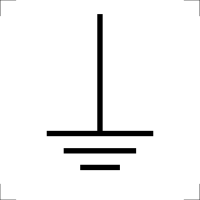
\includegraphics{part01/chap01/ground.png}
	\caption{Symbole représentant la terre \\ norme IEC 60417 }
\end{figure}

\index{terre}
\index{ground}

\section{La tension}

\begin{tabular}{ll}
\textbf{Notation usuelle~:} & $U$, $u$, $U_{AB}$ \\
\textbf{Unité~:} & Volt (V) \\
\textbf{Unité SI~:} & ${kg} \cdot m^2 \cdot {s}^{-3} \cdot A^{-1}$ \\
\textbf{Nature~:} & Grandeur scalaire \\
\end{tabular} 

\subsection*{Définition}

Une \keyword{tension} $U_{AB}$ est la circulation du champs électrique le long d'un circuit $\mathscr{C}$ entre les points $A$ et $B$~:

\begin{equation}
	U_{AB} = \int_{\mathscr{C}_{A}}^{\mathscr{C}_B}\vec{E}\,dl
\end{equation}

Cependant, cette définition est trop détaillée pour l'électronique. En effet, si l'on suppose que le temps de propagation des ondes électromagétiques est négligeable (hypothèse du régime stationnaire), la tension est alors égale à la "\textbf{différence de potentiel}" entre les deux extrémités du circuit.

\begin{equation}
	U_{AB} = V_A - V_B
\end{equation}

\index{potentiel!difference de potentiel@différence de potentiel}

\subsection*{Représentation graphique: }

\begin{minipage}{7cm}
\begin{center}
\includesvg{part01/chap01/tension}
\end{center}
\end{minipage}
\hspace{1cm}
\begin{minipage}{7cm}
Une tension est représentée par une flêche. Son sens est important car une tension est une \underline{grandeur signée}. 
\end{minipage}\\

\subsection*{Mesure d'une tension}

En électronique, une tension se mesure toujours \emph{entre deux points}, à l'aide d'un voltmètre (ou d'un oscilloscope si on veut en voir les variations temporelles). \\


\begin{minipage}{7cm}
\begin{center}
\includesvg{part01/chap01/mesure_tension}
\end{center}
\end{minipage}
\hspace{1cm}
\begin{minipage}{7cm} 
	Le voltmètre se connecte en parallèle de la tension à mesurer. 
\end{minipage}\\

\section{Le courant}

\begin{tabular}{ll}
\textbf{Notation usuelle~:} & $I$, $i$ \\
\textbf{Unité~:} & Ampère (A) \\
\textbf{Unité SI~:} & $A$ \\
\textbf{Nature~:} & Grandeur scalaire \\
\end{tabular} 

\subsection*{Définition}

Un \textbf{courant} est un mouvement d'ensemble de porteurs de charges électriques au sein d'un matériau conducteur. Ces porteurs de charge sont dans le cas le plus courant des électrons, mais cela peut également être des ions positifs ou négatifs (Par exemple dans le cas des electrolytes) ou encore n'importe quel corps portant une charge non nulle. 

\index{courant!courant électrique}

\subsection*{ Représentation graphique: }

\begin{minipage}{7cm}
	\includesvg{part01/chap01/courant} 
\end{minipage}
\hspace{1cm}
\begin{minipage}{7cm}
	Le courant électrique est généralement représenté par une flêche située sur le circuit. Son sens est important car un courant est une \underline{grandeur signée}. 
\end{minipage}\\

\subsection*{Mesure d'un courant électrique }

En pratique, un courant se mesure généralement à l'aide d'un ampèremètre. \\ 

\begin{minipage}{7cm}
\begin{center}
\includesvg{part01/chap01/mesure_courant}
\end{center}
\end{minipage}
\hspace{1cm}
\begin{minipage}{7cm} 
	L'ampèremètre se connecte en série sur le circuit dans lequel on veut mesurer un courant. 
\end{minipage}\\

\index{courant!mesure du courant}
\index{amperemetre@ampèremètre}

\subsection*{ Sens conventionnel du courant: }

Par convention, le courant sort du générateur électrique par la borne positive et y revient par la borne négative. C'est ce que l'on appelle le \textbf{sens conventionnel du courant}. \\
\index{courant!sens conventionnel du courant}
\index{conventionnel!sens conventionnel du courant}

On ne raisonne jamais en électronique en utilisant le sens réel des porteurs de charges, car celui-ci sera différent s'il s'agit d'électrons (qui circulent du pôle négatif vers le pôle positif du générateur) ou de cations (qui circulent en sens inverse). Cela n'a aucune importance et ne ferait que complexifier inutilement les raisonnements. Dans la suite de ce document, et plus largement dans l'intégralité des ouvrages lus par votre serviteur, c'est toujours le sens conventionnel qui est utilisé.

\subsection*{Intensité du courant}

L'\keyword{intensité} du courant électrique (parfois appelée "\keyword*{ampérage}" ou "\keyword*{courant}") correspond au débit de charges électriques à travers une surface donnée (le plus souvent la section d'un fil électrique)~: 

\begin{equation}
	i(t) = \dfrac{dq}{dt} 
\end{equation}

avec~: \\
\begin{itemize}
	\item[$\bullet$] $i$ : l'intensité du courant
	\item[$\bullet$] $q$ : la charge électrique
	\item[$\bullet$] $t$ : le temps.
\end{itemize}

\section{L'énergie électrique}

\begin{tabular}{ll}
\textbf{Notation usuelle~:} & $E$ \\
\textbf{Unité~:} & Joule (J) \\
	\textbf{Unité SI~:} & $kg \cdot m^2 \cdot s^{-2}$ \\
\textbf{Nature~:} & Grandeur scalaire \\
\end{tabular} 

\subsection*{Définition}

\textbf{Parler d'énergie électrique est au sens strict un abus de langage}. Ce n'est pas une véritable forme d'énergie comme peuvent l'être l'énergie cinétique ou l'énergie potentielle. Il s'agit plutôt d'un vecteur énergétique, c'est à dire un moyen de transférer de l'énergie entre deux systèmes : l'électricité requiert et transporte de l'énergie.\\
\index{energie@énergie}

L'énergie électrique est définie de la façon suivante~:

\begin{equation}
	E = q \cdot U
\end{equation}

avec~:\\
\begin{itemize}
	\item[$\bullet$] $E$ la quantité d'énergie en joules
	\item[$\bullet$] $q$ la charge électrique en coulombs
	\item[$\bullet$] $U$ la tension électrique en volts
\end{itemize}

\subsection*{Autre unité de mesure}

Le joule étant une unité de mesure assez petite pour les besoins des électriciens, une autre unité est souvent utilisée~: le kiloWattheure (kWh). 
\index{kiloWattheure}

$$ 1\:kWh = 10^3 \cdot 3600\:J = 3.6\:MJ $$


\subsection*{Lien avec la puissance}

si $I$ est le courant, la quantité de charges qui circulent pendant un temps $\Delta t$ est~: 

$$q = I \cdot \Delta t$$

(On suppose le courant constant pendant l'intervalle de temps).\\

La quantitée d'énergie échangée $E$ pendant $\Delta t$ est donc~:

$$ E = q \cdot U = I \cdot \Delta t \cdot U = U \cdot I \cdot \Delta t $$

Ce qui amène à~: \\
\begin{equation}
E = P \cdot \Delta t 
\end{equation}

avec $P$ la puissance électrique.

\section{La puissance électrique}

\begin{tabular}{ll}
\textbf{Notation usuelle~:} & $P$ \\
\textbf{Unité~:} & Watt (W) \\
	\textbf{Unité SI~:} & $kg \cdot m^2 \cdot s^{-3}$ \\
\textbf{Nature~:} & Grandeur scalaire \\
\end{tabular} 

\subsection*{Définition}

\textbf{La puissance électrique}\index{puissance!puissance electrique@puissance électrique} est un taux d'énergie transférée par un circuit électrique par unité de temps. La puissance est donc reliée à l'énergie échangée par la relation~:

\begin{equation}
	P = \dfrac{E}{\Delta t}
\end{equation}

Ce qui nous permet également de l'exprimer en fonction de la tension et du courant :

\begin{equation}
	P = U \cdot I
\end{equation}

Pour un générateur, cette quantité est négative (le générateur fournit de l'énergie). Pour une charge, cette quantité est positive.


\chapter{Les circuits électriques}

\section{Circuit électrique}

\index{circuit!circuit électrique@circuit électrique}
\index{potentiel!difference de potentiel@différence de potentiel}
\index{stationnaire!hypothèse du régime stationnaire}
\index{hypothèse!hypothèse du régime stationnaire}
\index{conducteur!conducteur parfait}

Si l'on a un regard de physicien sur un schéma électronique, il devient très difficile de réfléchir sur un circuit tant les choses sont complexes. Les ondes électromagnétiques se propagent dans les conducteurs selon des lois difficiles à appréhender, et il se passe bien des choses entre et dans chaque composant. L'électronique repose donc sur quelques hypothèses de simplification nous permettant de raisonner simplement.  

La première de ces hypothèses est l'\textbf{hypothèse du régime stationnaire}. Celle-ci implique que la propagation des ondes électromagnétiques est supposée terminée, et que nous pouvons négliger les effets qui en découlent. Ceci à deux conséquences : 

\begin{itemize}
\item \textbf{La tension est assimilée à la différence de potentiel} \\
\item \textbf{Dans un conducteur parfait (de résistance nulle), la différence de potentiel est nulle.}
\end{itemize}

\index{blocs!blocs fonctionnels}
\index{lumped!lumped elements}
\index{elements!lumped elements}
La seconde hypothèse importante est celle des \textbf{blocs fonctionnels} ("lumped elements" en anglais)~: ceci consiste à considérer que l'on peut représenter un circuit comme un ensemble de blocs simples (résistance, capacité, inductance, etc.) reliés entre eux par un réseau de fils parfaitement conducteurs.

Sauf mention contraire (Par exemple quand nous nous intéresserons aux radiofréquences pour lesquelles on ne peut plus négliger la propagation des ondes), nous supposerons toujours ces hypothèses valides.

\pagebreak
\section{Les dipôles}

\index{dipole@dipôle}
Un \textbf{dipôle}, comme son nom l'indique, est un composant dôté de deux bornes. On peut citer comme exemple de dipôle les résistances, les condensateurs, les bobines, les diodes, etc. Le problème est alors que les tensions, tout comme les intensités, sont des grandeurs signées. Afin de pouvoir caractériser un composant, il nous faut donc se mettre d'accord sur la manière de les choisir.

\subsection*{Convention recepteur}

\index{recepteur@récepteur}
\index{convention!convention recepteur@convention récepteur}
\index{recepteur@récepteur!convention recepteur@convention récepteur}
\index{dipole@dipôle!dipole recepteur@dipôle récepteur}
Pour les dipôles récepteurs, c'est à dire les dipôles prenant de l'énergie au circuit, la convention adoptée est la \textbf{convention récepteur}. Elle consiste à placer les flêches de tension et de courant dans des sens opposés. 

\begin{figure}[!h]
\centering
\includesvg{part01/chap02/convention_recepteur}
\caption{Dipôle en convention récepteur}
\end{figure}

Les différentes lois que nous allons écrire pour les composants (la loi d'Ohm par exemple) seront exprimées selon cette convention.

\subsection*{Convention générateur}

\index{generateur@générateur}
\index{convention!convention generateur@convention générateur}
\index{generateur@générateur!convention generateur@convention générateur}
\index{dipole@dipôle!dipole generateur@dipôle générateur}
Pour les dipôles générateurs, c'est à dire les dipôles fournissant de l'énergie au circuit, la convention adoptée est la \textbf{convention générateur}. Elle consiste à placer les flêches de tension et de courant dans le même sens. 

\begin{figure}[!h]
\centering
\includesvg{part01/chap02/convention_generateur}
\caption{Dipôle en convention générateur}
\end{figure}

Les différentes lois que nous allons écrire pour les générateurs (batteries, piles, sources de signal, etc.) seront exprimées selon cette convention.

\subsection*{Signe de la puissance électrique}

\index{puissance!puissance electrique@puissance électrique}
\index{puissance!convention generateur@convention générateur}
\index{puissance!convention recepteur@convention récepteur}
\index{puissance!signe}
Dans l'expression du calcul de la puissance, $P=U \cdot I$, le signe du résultat va donc dépendre de la convention utilisée.

\begin{table}[!h]
\begin{center}
\bgroup
\def\arraystretch{1.5}%  1 is the default, change whatever you need
\rowcolors{2}{blue!30}{blue!10}
\begin{tabular}{|c|c|c|}
	\hline
	& \textbf{Convention Récepteur} & \textbf{Convention Générateur} \\
	\hline
	Récepteur physique  & $P<0$ & $P>0$ \\
	\hline
	Générateur physique & $P>0$ & $P<0$ \\
	\hline
\end{tabular}
\egroup
\end{center}
	\caption{ Signe de la puissance }
\end{table}

\section{Lois de Kirchhoff}
\index{kirchhoff}
\index{kirchhoff!lois de Kirchhoff}
\textbf{Les lois de Kirchhoff} expriment la conservation de l'énergie et de la charge dans un circuit électrique. Au nombre de deux (la loi des noeuds et la loi des mailles), elles permettent de déterminer les valeurs courants et les tensions dans le circuit.

\subsection*{Loi des noeuds}
\index{kirchhoff!loi des noeuds}
\index{noeud!loi des noeuds}
\index{courant!loi des noeuds}
\index{noeud}
\vspace{0.5cm}
\begin{minipage}{3cm}
\begin{center}
\includesvg{part01/chap02/loi_des_noeuds}
\end{center}
\end{minipage}
\hspace{1cm}
\begin{minipage}{10cm} 
\textbf{La somme des intensités des courants qui entrent par un noeud est égale à la somme des intensités des courants qui sortent du même noeud.} \\
	$$ I_2 + I_3 = I_1 + I_4 $$
\end{minipage}\\

\smallskip
Cette loi découle directement de la conservation de la charge électrique, en tenant compte du fait qu'en régime stationnaire, ces charges ne peuvent pas s'accumuler à un endroit quelconque du circuit. Pour un noeud, cela veut donc dire que la quantité de charge entrante est égale à la quantité de charges sortantes.\\

\subsection*{Loi des mailles}
\index{kirchhoff!loi des mailles}
\index{tension!loi des mailles}
\index{maille!loi des mailles}
\index{maille}
\vspace{0.5cm}
\begin{minipage}{3cm}
\begin{center}
\includesvg{part01/chap02/loi_des_mailles}
\end{center}
\end{minipage}
\hspace{1cm}
\begin{minipage}{10cm} 
\textbf{Dans une maille quelconque d'un circuit, la somme des différences de potentiel le long de la maille est nulle.} \\

\hspace{1cm}
\begin{minipage}{8cm} 
Exemple~:
\begin{center}
$  U_1 - U_2 - U_3 - U_4 + U_6 = 0$ (Maille 1) 
\end{center}
Ou pour la maille passant par $U_5$~:
\begin{center}
$ U_1 - U_2 -U_3 - U_5 + U_6 = 0 $
	\end{center}
\end{minipage}\\
\end{minipage}\\

\smallskip
Cette loi est valable dans l'approximation des régimes stationnaires, et à condition que les variations de flux magnétique à travers la maille soient négligeables.

\section{Théorème de Millman}

\textbf{Le théorème de Millman} est une variante de la loi des noeuds, écrite sous la forme de potentiels. Il s'énonce de la façon suivante~:\\

\index{millman!theoreme de millman@théorème de Millman}
\index{noeud!theoreme de millman@théorème de Millman}
\index{potentiel!theoreme de millman@théorème de Millman}
\vspace{0.5cm}
\begin{minipage}{5cm}
\begin{center}
\includesvg{part01/chap02/millman}
\end{center}
\end{minipage}
\hspace{1cm}
\begin{minipage}{10cm}

	\textbf{Pour un noeud $M$, auquel sont connectées des branches contenant des résistances $R_i$ reliées à des potentiels $V_i$, le potentiel $V_M$ s'écrit~:}

\begin{equation}
	V_M = \dfrac{\displaystyle\sum_{i}\dfrac{V_i}{R_i}}{\displaystyle\sum_{i} \dfrac{1}{R_i} }
\end{equation}

\end{minipage}\\

\smallskip
Ce théorème peut également s'écrire avec des tensions (différences de potentiel).


\chapter{ Les dipôles idéaux }

\index{dipole@dipôle!dipole ideal@dipôle idéal}
\index{courant!caracteristique courant tension@caractéristique courant tension}
\index{tension!caracteristique courant tension@caractéristique courant tension}
Les \textbf{dipôles idéaux} correspondent à des relations entre la tension à leurs bornes et le courant qui les traverse (On parle de "\textbf{caractéristique courant/tension}"). Comme leur nom le laisse supposer, ces dipôles sont des représentations idéales des composants réels. Nous nous en servirons comme briques de base afin de modéliser les circuits. 

\section{Les générateurs idéaux}

\index{generateur@générateur}
\index{generateur@générateur!generateur ideal@générateur idéal}
\subsection{ Le générateur de tension }

\index{generateur@générateur!generateur de tension@générateur de tension}
\index{tension!generateur de tension@générateur de tension}
Un \textbf{générateur idéal de tension} est un générateur dont la tension est constante, et ce quel que soit le courant demandé.

\begin{figure}[!h]
\begin{center}
\includesvg[scale=0.7]{part01/chap03/generateur_ideal_tension}
\hspace{1cm}
\includesvg[scale=0.7]{part01/chap03/carac_generateur_ideal_tension}
\end{center}
\caption{ Symbole et caractéristique courant/tension du générateur idéal de tension}
\end{figure}

Le générateur de tension ne peut être que théorique car mis en court-circuit, il devrait délivrer un courant infini et donc fournir au circuit une puissance également infinie.\\

Cette définition du générateur idéal de tension est parfois étendue à des générateurs dont la tension est une fonction du temps $u(t)$. Dans ce cas, la tension fournie ne dépendra que du temps et pas du courant. 

\subsection{ Le générateur idéal de courant }

\index{generateur@générateur!generateur de courant@générateur de courant}
\index{courant!generateur de courant@générateur de courant}
Un \textbf{générateur idéal de courant} est un générateur fournissant un courant constant, et ce quel que soit la tension appliquée à ses bornes.

\begin{figure}[!h]
\begin{center}
\includesvg[scale=0.7]{part01/chap03/generateur_ideal_courant}
\hspace{1cm}
\includesvg[scale=0.7]{part01/chap03/carac_generateur_ideal_courant}
\end{center}
\caption{ Symbole et caractéristique courant/tension du générateur idéal de courant}
\end{figure}

Tout comme le générateur idéal de tension, c'est un générateur théorique car dans le cas du circuit ouvert il fournirait une tension infinie.\\

Ici encore, on peut étendre cette définition à des générateurs dont le courant n'est pas constant, mais une fonction du temps $I(t)$. Dans ce cas, le courant fourni ne dépendra que du temps et pas de la tension appliquée aux bornes du générateur.


\section{ Les dipôles linéaires }

\index{dipole@dipôle!dipole linéaire@dipôle linéaire}
\index{resistor@résistor}
\index{bobine}
\index{condensateur}
On parle de \textbf{dipôles "linéaires"} (ce qui est un petit abus de langage) pour désigner les dipôles possédant une relation linéaire entre~:\\
\begin{itemize}
\item tension et courant, 
\item tension et charge électrique,
\item ou courant et dérivée de la tension.\\
\end{itemize}

Ces dipôles linéaires sont au nombre de trois~: \\

\begin{itemize}
\item \textbf{La résistance}
\item \textbf{L'inductance}
\item \textbf{La capacité} \\
\end{itemize}

Il faut bien faire la différence entre ces trois dipôles idéaux et leurs "incarnations" en composants que sont les résistors, les bobines et les condensateurs. \\

\subsection{ La résistance }

\index{resistance@résistance}
\index{ohm}
\vspace{0.5cm}
\begin{tabular}{ll}
\textbf{Notation usuelle~:} & $R$ \\
\textbf{Unité~:} & Ohm ($\Omega$) \\
\textbf{Unité SI~:} & $m^2 \cdot kg \cdot {s}^{-3} \cdot A^{-2}$ \\
\textbf{Nature~:} & Grandeur scalaire \\
\end{tabular} 

\subsubsection*{Définition}

La \textbf{résistance} traduit une relation linéaire entre courant et tension. Le symbole qui permet de la représenter est généralement l'un des deux suivants~:

\index{resistance@résistance!symbole}
\begin{figure}[!h]
\centering
\begin{subfigure}{.4\textwidth}
\centering
	\includesvg[width=0.8\textwidth]{part01/chap03/symbole_r_euro}
\caption{Symbole Euro}
\end{subfigure}%
\begin{subfigure}{.4\textwidth}
\centering
	\includesvg[width=0.8\textwidth]{part01/chap03/symbole_r_us} 
\caption{Symbole US}
\end{subfigure}
\caption{Symbole de la résistance}
\end{figure}

\index{resistance@résistance!loi d'Ohm}
\index{ohm!loi d'Ohm}
Le comportement courant/tension d'une résistance est défini par la \textbf{loi d'Ohm}~:\\
\begin{center}
\begin{minipage}{.2\textwidth}
\begin{center}
\includesvg{part01/chap03/carac_R}
\end{center}
\end{minipage}
\hspace{1cm}
\begin{minipage}{.3\textwidth} 
\begin{equation}
	I_R = \dfrac{U_R}{R}
\end{equation}
\end{minipage}
\end{center}

avec~:\\

\begin{itemize}
\item $U_R$ La tension aux bornes de la résistance
\item $I_R$ Le courant traversant la résistance
\item $R$ La valeur de la résistance en Ohms\\
\end{itemize}


Lorsqu'un conducteur montre une caractéristique courant/tension vérifiant la loi d'Ohm (une droite passant par l'origine), on parle de "\textbf{Conducteur ohmique}". On utilise parfois également les termes de "\textbf{résistance pure}" ou "\textbf{résistance idéale}".

\index{conducteur!conducteur ohmique}
\index{resistance@résistance!resistance pure@résistance pure}
\index{resistance@résistance!resistance ideale@résistance idéale}
\subsubsection*{Effet Joule}

Physiquement, le courant est un mouvement de porteurs de charge. Or dans un conducteur ohmique, ces porteurs interagissent avec les atomes constitutifs du milieu dans lequel ils se déplacent, ce qui constitue un frein à leur mouvement. Ceci se traduit par l'\textbf{effet~Joule}. C'est un effet thermique qui provoque une augmentation de l'énergie interne du conducteur, et généralement de sa température. \\

\index{Joule!resistance ideale@effet Joule}
L'énergie dissipée sous forme de chaleur entre deux instants $t_1$ et $t_2$ par un dipôle de résistance $R$ lorsque circule un courant d'intensité $i$ s'écrit~:

$$ Q_{joule} = R \int_{t_1}^{t_2} i^2\,dt $$

La puissance moyenne s'écrit alors~:

$$ P = \dfrac{Q_{joule}}{t_2 - t_1} = \dfrac{R}{t_2 - t_1} \int_{t_1}^{t_2}i^2\,dt $$\\

Dans le cas d'un courant \underline{constant} $I$, l'expression devient alors~:

\begin{equation}
	P = R\,I^2
\end{equation}

\subsubsection*{Résistance équivalente}

\index{resistance@résistance!resistance equivalente@résistance équivalente}
La \textbf{résistance équivalente} consiste à remplacer dans une partie du circuit un ensemble de résistances par une seule, qui doit être équivalente (dans le sens où le comportement du circuit doit être le même).\\ 

\begin{itemize}
\item \underline{Association en série} : La résistance du dipôle équivalent vaut la somme des résistances de chacun des dipôles. \\

\index{resistance@résistance!association en serie@association en série}
\begin{center}
\begin{minipage}{.2\textwidth}
\begin{center}
\includesvg{part01/chap03/r_serie}
\end{center}
\end{minipage}
\hspace{1cm}
\begin{minipage}{.3\textwidth} 
\begin{equation}
	R_{eq} = R_1 + R_2
\end{equation}
\end{minipage}
\end{center}

\vspace{0.5cm}

\item \underline{Association en parallèle} : l'inverse de la résistance du dipôle équivalent vaut la somme des inverses des résistances de chacun des dipôles. \\

\index{resistance@résistance!association en parrallele@association en parallèle}
\begin{center}
\begin{minipage}{.2\textwidth}
\begin{center}
	\includesvg{part01/chap03/r_parallele}
\end{center}
\end{minipage}
\hspace{1cm}
\begin{minipage}{.3\textwidth} 
\begin{equation}
	\dfrac{1}{R_{eq}} = \dfrac{1}{R_1} + \dfrac{1}{R_2} 
\end{equation}
\end{minipage}
\end{center}
\end{itemize}

\subsection{ La capacité électrique }

\index{capacite@capacité!capacite electrique@capacité électrique}
\index{farad}
\vspace{0.5cm}
\begin{tabular}{ll}
\textbf{Notation usuelle~:} & $C$ \\
\textbf{Unité~:} & Farad (F) \\
	\textbf{Unité SI~:} & $m^{-2} \cdot kg^{-1} \cdot {s}^{4} \cdot A^{2}$ \\
\textbf{Nature~:} & Grandeur scalaire \\
\end{tabular} 

\subsubsection*{Définition}

\index{charge!charge electrique@charge électrique}
La \textbf{capacité électrique} est l'aptitude d'un conducteur ou d'un dipôle à stocker une charge électrique en réponse à une différence de potentiel. Elle est exprimée sous la forme d'un ratio entre ces deux quantités. La capacité traduit donc une relation linéaire entre charge et différence de potentiel~:

\begin{equation}
	Q = C\,U
\end{equation}

avec~:\\
\begin{itemize}
	\item $Q$ la charge stockée
	\item $C$ la capacité électrique
	\item $U$ la différence de potentiel\\
\end{itemize}

\index{capacite@capacité!capacite propre@capacité propre}
\index{capacite@capacité!capacite mutuelle@capacité mutuelle}
\index{capacitance@self capacitance}
\index{capacitance@mutual capacitance}
En physique, on distingue généralement la "\textbf{capacité propre}" (self capacitance) de la "\textbf{capacité mutuelle}" (mutual capacitance). Un objet qui peut être chargé électriquement montre une capacité propre : on mesure alors le potentiel électrique par rapport à la terre. La capacité mutuelle, elle, est mesurée entre deux objets différents. Par exemple entre les deux armatures d'un condensateur. 

\subsubsection{ Note à propos du farad~: }

\index{farad}
L'unité utilisée pour la capacité électrique, le farad, est très grande ! En pratique, on en utilise le plus souvent des sous-multiples : le microfarad ($\mu F$), le nanofarad ($nF$) ou le picofarad ($pF$). 


\subsubsection{ Relation Courant-Tension~: }

\index{capacite@capacité!caracteristique courant tension@caractéristique courant tension}
Si on note $Q$ la charge de l'armature positive du condensateur parfait, on a bien~:

$$Q = C\,U_C$$

Ce qui en dérivant par le temps, donne~:

$$\dfrac{dQ}{dt} = C\,\dfrac{dU_C}{dt}$$

En revenant à la définition du courant, on reconnait dans la partie gauche de l'équation l'écriture de l'intensité. On a alors~:

\begin{equation}
	I_C = C\,\dfrac{dU_C}{dt}
\end{equation}

\subsubsection{Le condensateur idéal}

\index{condensateur!condensateur ideal@condensateur idéal}
Le condensateur idéal est un dipôle au comportement purement capacitif, formé de deux armatures conductrices parallèles séparées par un isolant, le diéléctrique. On le représente à l'aide du symbole suivant~:

\begin{figure}[!h]
\centering
\includesvg{part01/chap03/symbole_c}
\caption{Symbole du condensateur simple}
\end{figure}

\subsubsection{ Capacité équivalente~: }

\index{condensateur!condensateur equivalent@condensateur équivalent}
\index{capacite@capacité!capacite equivalente@capacité équivalente}
Tout comme pour les résistances, on définit la \textbf{capacité équivalente} qui consiste à remplacer un ensemble de capacités par une seule.\\ 

\begin{itemize}
\item \underline{Association en série} : \\

\index{capacite@capacité!association en serie@association en série}
\begin{center}
\begin{minipage}{.2\textwidth}
\begin{center}
\includesvg{part01/chap03/c_serie}
\end{center}
\end{minipage}
\hspace{1cm}
\begin{minipage}{.3\textwidth} 
\begin{equation}
	\dfrac{1}{C_{eq}} = \dfrac{1}{C_1} + \dfrac{1}{C_2}
\end{equation}
\end{minipage}
\end{center}

\vspace{0.5cm}

\item \underline{Association en parallèle} : \\

\index{capacite@capacité!association en parallele@association en parallèle}
\begin{center}
\begin{minipage}{.2\textwidth}
\begin{center}
	\includesvg{part01/chap03/c_parallele}
\end{center}
\end{minipage}
\hspace{1cm}
\begin{minipage}{.3\textwidth} 
\begin{equation}
	C_{eq} = C_1 + C_2
\end{equation}
\end{minipage}
\end{center}
\end{itemize}


\subsection{ L'inductance }

\index{inductance}
\index{Henry}
\vspace{0.5cm}
\begin{tabular}{ll}
\textbf{Notation usuelle~:} & $L$ \\
\textbf{Unité~:} & Henry (H) \\
	\textbf{Unité SI~:} & $m^2 \cdot kg \cdot {s}^{-2} \cdot A^{-2}$ \\
\textbf{Nature~:} & Grandeur scalaire \\
\end{tabular} 

\subsubsection*{Définition}

\index{inductance}
L'\textbf{inductance} est la tendance d'un conducteur électrique à s'opposer à tout changement du courant le traversant. \\

Lorsqu'un courant electrique parcourt un conducteur, un champs magnétique se crée autour de ce conducteur. La force de ce champs magnétique dépend de l'amplitude du courant et en suit donc les changements. Cependant, d'après la loi de Faraday, tout changement d'un champs magnétique induit une force electromotrice (tension) dans le conducteur. Cette tension induite créée par le changement de courant a pour effet de s'opposer à ce dernier. \\

\subsubsection{Relation Courant-Tension}

\index{inductance!caracteristique courant tension@caractéristique courant tension}
\index{EMF!back-EMF}
\index{force!force contre-electromotrice}
\index{auto-inductance}
\index{inductance!auto-inductance}
Comme le veut la loi d'Ampère, un courant $i$ circulant dans un conducteur génère un champs magnétique $\vec{B}$ autour de ce conducteur. Le flux $\Phi$ de ce champs magnétique au travers du circuit $C$ est égal à l'intégrale suivante : 

$$\Phi = \iint_{C}{\vec{B}.\vec{dA}}$$ 

Si le courant varie, le flux magnétique $\Phi$ varie également. Or d'après la loi de Faraday, tout changement dans le flux magnétique au travers d'un circuit induit dans ce dernier une force électromotrice ($ \varepsilon $)~:

$$ \varepsilon (t) = - \,\dfrac{d}{dt} \Phi(t) $$

Le signe moins dans cette équation nous indique que le voltage induit est dans une orientation qui tend à s'opposer au changement de courant. On l'appelle souvent pour cette raison "\textbf{force contre-electromotrice}" ou "\textbf{back-EMF}".\\

L'{auto-inductance}, plus généralement nommée "inductance" $L$, est le ratio entre le voltage induit et le changement de courant. En convention récepteur, on a la relation :

\begin{equation}
	U_L = L \, \dfrac{dI_L}{dt}
\end{equation}

\subsubsection{ Inductance idéale }
\index{bobine!bobine simple}
\index{bobine!bobine ideale@bobine idéale}
\index{inductance!inductance ideale@inductance idéale}
On définit l'inductance, aussi appelée \textbf{bobine simple} ou \textbf{bobine idéale}, comme un dipôle au comportement purement inductif ( les effets capacitifs et ohmiques sont donc négligés ). On la représente à l’aide du symbole suivant :

\begin{figure}[!h]
\centering
\includesvg{part01/chap03/symbole_l}
	\caption{Symbole de l'inductance}
\end{figure}

\index{inductance!symbole}
I\subsubsection{ Inductance équivalente~: }

\index{inductance!inductance equivalente@inductance équivalente}
Le calcul de l'\textbf{inductance équivalente} se fait de façon similaire à celle des résistances~:\\ 

\begin{itemize}
\item \underline{Association en série} : \\

\index{inductance!association en serie@association en série}
\begin{center}
\begin{minipage}{.2\textwidth}
\begin{center}
\includesvg{part01/chap03/l_serie}
\end{center}
\end{minipage}
\hspace{1cm}
\begin{minipage}{.3\textwidth} 
\begin{equation}
	L_{eq} = L_1 + L_2
\end{equation}
\end{minipage}
\end{center}

\vspace{0.5cm}

\item \underline{Association en parallèle} : \\
\index{inductance!association en parrallele@association en parrallèle}

\begin{center}
\begin{minipage}{.2\textwidth}
\begin{center}
	\includesvg{part01/chap03/l_parallele}
\end{center}
\end{minipage}
\hspace{1cm}
\begin{minipage}{.3\textwidth} 
\begin{equation}
	\dfrac{1}{L_{eq}} = \dfrac{1}{L_1} + \dfrac{1}{L_2}
\end{equation}
\end{minipage}
\end{center}
\end{itemize}




\chapter{Les circuits linéaires}

\index{circuit!circuit lineaire@circuit linéaire}
On appelle "\textbf{circuit linéaire}" tout circuit formé uniquement de dipôles linéaires (résistance, capacités et inductances) et de sources de tension ou de courant indépendantes. \\

Les circuits linéaires sont une grande famille de circuits particulièrement faciles à manipuler, car cette propriété de linéarité nous donne des théorèmes très utiles :\\

\begin{itemize}
\item Le théorème de superposition
\item Le théorème de Thévenin
\item Le théorème de Norton
\end{itemize}


\section{Théorème de superposition}

\index{theoreme@théorème!theoreme de superposition@théorème de superposition}
\index{theoreme@théorème!theoreme de helmotz@théorème de Helmotz}
Le \textbf{théorème de superposition}, ou "\textbf{théorème de Helmotz}" est rendu possible par la linéarité des équations régissant cette famille de circuit. Il s'exprime en ces termes~:\\

\textbf{Dans un circuit linéaire avec plusieurs sources, le courant et la tension pour tout élément du circuit est la somme des courants et des tensions produits par chaque source agissant indépendamment.} \\

Pour appliquer ce théorème, on calcule la contribution de chacune des sources de tension ou de courant au résultat final en "éteignant" toutes les autres sources.\\

Pour "éteindre" une source de tension, on la remplace par un fil. \\

Pour "éteindre" une source de courant, on la remplace par un circuit ouvert. \\

On somme ensuite toutes les contributions pour obtenir le résultat final.

\pagebreak
\subsubsection*{Exemple~:}

On cherche la valeur de la tension $U_{AB}$ dans le circuit suivant~:

\begin{center}
	\includesvg[scale=0.8]{part01/chap04/superposition}
\end{center}


\subsubsection*{Calcul de la contribution de $U_G$}


On "éteint" tous les générateurs à l'exception du générateur de tension $U_G$. Le circuit devient alors~:

\begin{center}
	\includesvg[scale=0.8]{part01/chap04/superposition_2}
\end{center}

On peut alors le réarranger afin de le rendre plus facilement lisible~:

\begin{center}
	\includesvg[scale=0.8]{part01/chap04/superposition_3}
\end{center}

Le courant débité par le générateur $U_G$ s'écrit alors :

$$ I = \dfrac{U_G}{R_1 + R_2} $$

Ce courant traversant la résistance $R_2$, on peut alors écrire~:

$$ U_{AB} = R_2 \, I = \dfrac{R_2}{R_1 + R_2} U_G $$

\subsubsection*{Calcul de la contribution de $I_G$}

On "éteint" cette fois-ci tous les générateurs à l'exception du générateur de courant. $U_G$ est donc remplacé par un fil :

\begin{center}
	\includesvg[scale=0.8]{part01/chap04/superposition_4}
\end{center}

Une fois réarrangé un peu, le schéma devient~:

\begin{center}
	\includesvg[scale=0.8]{part01/chap04/superposition_5}
\end{center}

En utilisant la résistance équivalente, il vient alors~:

$$ U_{AB} = R_{eq}\,I_G = \dfrac{R_1 R_2}{R_1 + R_2}\,I_G $$

\subsubsection*{Conclusion}

\begin{center}
	\includesvg[scale=0.8]{part01/chap04/superposition}
\end{center}

Pour obtenir la réponse finale, il suffit alors de sommer les contributions des différentes sources~:

$$ U_{AB} = \underbrace{\dfrac{R_2}{R_1 + R_2} U_G}_{Contribution\,de\,U_G} + \underbrace{\dfrac{R_1 R_2}{R_1 + R_2}\,I_G}_{Contribution\,de\,I_G} $$

\pagebreak

\section{Théorème de Thévenin}

\index{theoreme@théorème!theoreme de thevenin@théorème de Thévenin}
\index{thevenin@thévenin!theoreme de thevenin@théorème de Thévenin}
Ce théorème découle des propriétés de linéarité des circuits considérés et donc du théorème de superposition. Il s'énonce de la façon suivante : \\

\textbf{"Un réseau électrique linéaire vu de deux points est équivalent à un générateur de tension parfait dont la force électromotrice est égale à la différence de potentiels à vide entre ces deux points, en série avec une résistance égale à celle que l'on mesure entre les deux points lorsque les générateurs indépendants sont rendus passifs."}

\begin{figure}[!h]
\begin{center}
	\includesvg{part01/chap04/thevenin}
\end{center}
\caption{Modèle de Thévenin}
\end{figure}
La tension $E_{Th}$ du générateur de Thévenin est égale à la tension à vide du montage, mesurée entre $A$ et $B$. \\

Pour trouver la résistance de Thévenin $R_{Th}$, on "éteint" tous les générateurs et on détermine la résistance équivalente entre $A$ et $B$.

\section{Théorème de Norton}

\index{theoreme@théorème!theoreme de norton@théorème de Norton}
\index{norton@norton!theoreme de norton@théorème de Norton}
De façon analogue, le \textbf{théorème de Norton} nous dit qu'il est possible de remplacer un circuit linéaire par un dipôle comprenant un générateur de courant et une résistance en parrallèle : 

\begin{figure}[!h]
\begin{center}
	\includesvg{part01/chap04/norton}
\end{center}
\caption{Modèle de Norton}
\end{figure}


Pour déterminer la valeur de $I_N$, on connecte un fil entre les points $A$ et $B$ et on détermine le courant traversant ce fil. \\

Pour déterminer la valeur de la résistance $R_N$, on procède de la même façon que pour le théorème de Thévenin : On éteint toutes les sources de courant ou de tension et on calcule la résistance équivalente entre $A$ et $B$.

\section{Equivalence entre Thévenin et Norton}

\index{norton@norton!equivalence norton thevenin@équivalence Norton Thévenin}
\index{thevenin@thévenin!equivalence thevenin norton@équivalence Thévenin Norton}
Les modèles de Thévenin et de Norton sont équivalents. Il est possible de passer de l'un à l'autre par la relation suivante~:

\begin{figure}[!h]
\begin{center}
\includesvg{part01/chap04/eq_thevenin_norton}
\end{center}
\caption{Equivalence entre les modèles de Thévenin et Norton}
\end{figure}

\section{Le diviseur de tension}

\index{diviseur!diviseur de tension}
\index{tension!diviseur de tension}
\index{pont!pont diviseur de tension}
Le \textbf{diviseur de tension}, aussi appelé "\textbf{pont diviseur}", est un circuit passif linéaire permettant de produire une tension de sortie $U_{out}$ qui est une fraction de la tension d'entrée $U_{in}$. Il se forme à l'aide de deux résistances~:

\begin{figure}[!h]
\begin{center}
\begin{minipage}{8cm}
	\includesvg[scale=0.9]{part01/chap04/diviseur_tension}
\end{minipage}
\begin{minipage}{8cm}

	\textbf{\underline{Pont diviseur à vide~:}}\\

	Si l'on suppose qu'aucun courant ne sort du pont diviseur~:
	\begin{equation}
		U_{out} = \dfrac{R_2}{R_1 + R_2}\,U_{in}
	\end{equation}
\end{minipage}
\end{center}
\caption{Diviseur de tension}
\end{figure}

Cette relation n'est cependant valable que si le courant sortant du pont diviseur est nul ou négligeable devant le courant traversant $R_2$. Si ce n'est pas le cas, on est alors dans le cas du \textbf{diviseur de tension chargé}~:\\


\begin{center}
	\includesvg[scale=0.9]{part01/chap04/diviseur_tension_load}
\end{center}

Le courant $I_{out}$ en sortie du pont diviseur n'est plus considéré comme négligeable. On utilise alors la résistance équivalente au couple $R_2$ et $R_L$ et la relation devient~:

$$ U_{out} = U_{in}\,\dfrac{R_{eq}}{R_1+R_{eq}} = U_{in} \, \dfrac{ R_2R_L }{R_1R_2 + R_1R_L + R_2R_L} $$


\section{Le diviseur de courant}

\index{diviseur!diviseur de courant}
\index{courant!diviseur de courant}
\index{pont!pont diviseur de courant}
La formule du \textbf{diviseur de courant} permet de calculer l'intensité du courant dans une résistance lorsque celle-ci fait partie d'un ensemble de résistances en parallèle et lorsque l'on connaît le courant total qui alimente cet ensemble. C'est le montage dual du diviseur de tension.


\begin{center}
\begin{minipage}{8cm}
	\includesvg[scale=0.9]{part01/chap04/diviseur_courant}
\end{minipage}
\begin{minipage}{8cm}

	Le courant qui traverse $R_1$ s'écrit~:
	$$	I_{1} = I \, \dfrac{\dfrac{1}{R_1}}{\dfrac{1}{R_1} + \dfrac{1}{R_2} + \dots + \dfrac{1}{R_n}} $$

	ou encore, exprimé avec les conductances~:

	$$ I_1 = I \, \dfrac{ G_1 } { G_1 + G_2 + \dots + G_n } $$
\end{minipage}\\
\end{center}

\vspace{5mm}

\begin{flushleft}
\textbf{\underline{Note:}} 
\end{flushleft}

\index{conductance}
La \textbf{conductance électrique} d'un matériau soumis à une différence de potentiel quantifie sa capacité à laisser passer un courant électrique. C'est une grandeur définie comme l'inverse de la résistance. Elle est généralement notée $G$ et exprimée en Siemens (S).


\chapter{ Analyse temporelle }

\section{Charge d'un condensateur}

Afin d'étudier la charge d'un condensateur, on utilise le montage RC suivant :

\begin{center}
\includesvg{part01/chap05/charge_c}
\end{center}

À l'instant $t=0$, la tension $U_{in}$ passe de 0V à $E_0$. \\

La loi des mailles donne :

$$U_{in} = U_R + U_C $$

Avec pour la résistance et pour le condensateur :

$$U_R = R\,I$$
$$ I = C \, \dfrac{d\,U_C}{dt} $$

Ce qui permet d'établir l'équation différentielle suivante pour $t>0$~:

$$ RC\,\dfrac{dU_C}{dt} + U_C = E_0 $$ \\

On introduit dans cette expression la constante de temps $\tau = RC$

La solution de l'équation différentielle (en tenant compte des conditions aux limites) est alors~:

$$ U_C(t) = E_0\,(\,1 - e^{-t/\tau}\,) $$

\begin{figure}[!h]
\begin{minipage}{13cm}
\begin{center}
\begin{gnuplot}[terminal=epslatex, terminaloptions=color dashed]
set key at 3,2 horizontal center
set key width 2
set key opaque
set sample 1000
set arrow from graph 0,1 to graph 0,1.05 size screen 0.025,15,60 filled ls -1
set xzeroaxis linetype -1
set xtics axis 
set ytics border nomirror
set border 2
set xr [-1.5:5]
set yr [-1:10]
set xlabel 't (s)'
set ylabel 'Volts'
set tmargin 1
set rmargin 2
R = 2000
C = 400e-6
Tau = R*C
E = 8
step(x) = x>0 ? E : 0
reponse(x) = x<0 ? 0 : E*(1-exp(-x/Tau)) 
plot step(x) w l lc 1 lw 3 t '$U_{in}$',\
reponse(x) w l lc 2 lw 3 t '$U_C$'
\end{gnuplot}
\end{center}
\end{minipage}
\begin{minipage}{3cm}
$E_0 = 8V$ \\
$R = 2\,k\Omega$ \\
$C = 400 \, \mu F$ \\
\bigskip
$ \tau = 0.8\,s $ \\
\end{minipage} \\
	\caption{Charge d'un condensateur}
\end{figure}

\subsection*{Influence de la constante de temps}
\smallskip
\begin{itemize}

\item Au bout d'un temps $3\tau$, la charge du condensateur est à $95\%$ de la valeur finale.

$$ U(3\tau) = E_0\,(\,1-e^{-3}_,) = 0.95 \, E_0$$ \\

\item Au bout d'un temps $5\tau$, la charge du condensateur est à $99.3\%$ de la valeur finale.

$$ U(5\tau) = E_0\,(\,1-e^{-5}_,) = 0.993 \, E_0$$ \\


\item La tangente à l'origine de la courbe coupe la valeur limite ($E_0$) en $t = \tau$

\end{itemize}

\pagebreak

\section{Décharge d'un condensateur}

Afin d'étudier la décharge d'un condensateur, on utilise le montage RC suivant :
\begin{center}
\includesvg{part01/chap05/decharge_c}
\end{center}
À l'instant $t=0$, la tension $U_{in}$ passe de $E_0$ à $0V$. La loi des mailles donne :
\begin{center}
$U_{in} = U_R + U_C$ avec $U_R = R\,I$ et $ I = C \, \dfrac{d\,U_C}{dt} $
\end{center}
Ce qui permet d'établir l'équation différentielle suivante pour $t>0$~:
$$ RC\,\dfrac{dU_C}{dt} + U_C = 0 $$ 
En posant $\tau = RC$, la solution de l'équation différentielle est alors~: $ U_C(t) = E_0\,e^{-t/\tau} $

\begin{figure}[!h]
\begin{minipage}{13cm}
\begin{center}
\begin{gnuplot}[terminal=epslatex, terminaloptions=color dashed]
set key at 3,2 horizontal center
set key width 2
set key opaque
set sample 1000
set arrow from graph 0,1 to graph 0,1.05 size screen 0.025,15,60 filled ls -1
set xzeroaxis linetype -1
set xtics axis 
set ytics border nomirror
set border 2
set xr [-1.5:5]
set yr [-1:10]
set xlabel 't (s)'
set ylabel 'Volts'
set tmargin 1
set rmargin 2
R = 2000
C = 400e-6
Tau = R*C
E = 8
step(x) = x>0 ? 0 : E
reponse(x) = x<0 ? E : E*exp(-x/Tau)
plot step(x) w l lc 1 lw 3 t '$U_{in}$',\
reponse(x) w l lc 2 lw 3 t '$U_C$'
\end{gnuplot}
\end{center}
\end{minipage}
\begin{minipage}{3cm}
$E_0 = 8V$ \\
$R = 2\,k\Omega$ \\
$C = 400 \, \mu F$ \\
\bigskip
$ \tau = 0.8\,s $ \\
\end{minipage} \\
	\caption{décharge d'un condensateur}
\end{figure}

\subsection*{Influence de la constante de temps}
\smallskip
\begin{itemize}

\item Au bout d'un temps $3\tau$, la charge du condensateur est à $5\%$ de la valeur initiale.

$$ U(3\tau) = E_0\,e^{-3} = 0.05 \, E_0$$ \\

\item Au bout d'un temps $5\tau$, la charge du condensateur est à $0.6\%$ de la valeur initiale.

$$ U(5\tau) = E_0\,e^{-5} = 0.006 \, E_0$$ \\

\item La tangente à l'origine de la courbe coupe la valeur 0 en $t = \tau$

\end{itemize}

\section{Établissement du courant dans une inductance}

On considère le schéma du circuit RL suivant :

\begin{center}
\includesvg{part01/chap05/echelon_l}
\end{center}

À l'instant $t=0$, la tension $U_{in}$ passe de 0V à $E_0$. \\

La loi des mailles donne :

$$U_{in} = U_R + U_L $$

Avec pour la résistance et pour le condensateur :

$$U_R = R\,I$$
$$ U_L = L \, \dfrac{d\,I}{dt} $$

Ce qui permet d'établir l'équation différentielle suivante pour $t>0$~:

$$ R\,I + L\,\dfrac{d\,I}{dt}   = E_0 $$ \\

On introduit dans cette expression la constante de temps $\tau = \dfrac{L}{R}$~:

$$ I + \dfrac{L}{R}\dfrac{d\,I}{dt}   = \dfrac{E_0}{R} $$ \\

Pour $t>0$, la solution de cette équation différentielle est~:

$$ I(t) = \dfrac{E_0}{R}\,(\,1 - e^{-t/\tau}\,) $$

Ce qui correspond à la tension $U_L$ suivante :

$$ U_L(t) = L \dfrac{d\,I}{d\,t} = E_0 \, e^{-t/\tau}\ $$


\begin{figure}[!h]
	\begin{center}
	\begin{gnuplot}[terminal=epslatex, terminaloptions={color dashed}]
set key horizontal outside bottom
set key width 2
set key opaque
set sample 1000
set arrow from graph 0,1 to graph 0,1.05 size screen 0.025,15,60 filled ls -1
set arrow from graph 1,1 to graph 1,1.05 size screen 0.025,15,60 filled ls -1
set xzeroaxis linetype -1
set xtics axis 
set ytics  border nomirror
set y2tics border nomirror
set border 10
set xr [-0.5:5.9]
set link y2 via y/10 inverse y*10
set yr [-1:10]
set xlabel 't (s)'
set ylabel 'Volts'
set y2label 'Ampères'
set tmargin 1
set rmargin 2
R = 8
L = 10
Tau = L/R
E = 8
step(x) = x>0 ? E : 0
tension(x) = x<0 ? 0 : E*exp(-x/Tau)
courant(x) = x<0 ? 0 : E/R*(1-exp(-x/Tau)) 
plot step(x) w l lc 1 lw 3 t '$U_{in}$',\
tension(x) w l lc 2 lw 3 t '$U_L$',\
courant(x) w l lc 3 lw 3 t '$I_L$' axis x1y2
\end{gnuplot} 
\begin{minipage}{\textwidth}
\bigskip
\begin{center}
$E_0 = 8V \quad R = 8\,\Omega \quad L = 10\,H \quad \tau = 1.25\,s $ 
\end{center}
\end{minipage}
\end{center}
\caption{Etablissement du courant dans un circuit RL}
\end{figure}

Les équations différentielles étant les mêmes, les remarques concernant la constante de temps $\tau$ effectuées dans les chapitres précédants restent valides. \\


\section{Rupture du courant dans une inductance}

On considère le circuit RL suivant :

\begin{center}
\includesvg{part01/chap05/echelon2_l}
\end{center}

À l'instant $t=0$, la tension $U_{in}$ passe de $E_0$ à $0V$. \\

La loi des mailles donne :

$$U_{in} = U_R + U_L $$

Avec pour la résistance et pour le condensateur :

$$U_R = R\,I$$
$$ U_L = L \, \dfrac{d\,I}{dt} $$ \\

Ce qui permet d'établir l'équation différentielle suivante pour $t>0$~:

$$ R\,I + L\,\dfrac{d\,I}{dt}   = 0 $$ 

On introduit dans cette expression la constante de temps $\tau = \dfrac{L}{R}$~:

$$ I + \dfrac{L}{R}\dfrac{d\,I}{dt}   = 0 $$ \\

Pour $t>0$, la solution de cette équation différentielle est~:

$$ I(t) = \dfrac{E_0}{R}\,e^{-t/\tau} $$  

\pagebreak

Ce qui correspond à la tension $U_L$ suivante :

$$ U_L(t) = L \dfrac{d\,I}{d\,t} = - E_0 \, e^{-t/\tau}\ $$

\begin{figure}[!h]
	\begin{center}
	\begin{gnuplot}[terminal=epslatex, terminaloptions={color dashed}]
set key horizontal outside bottom
set key width 2
set key opaque
set sample 1000
set arrow from graph 0,1 to graph 0,1.05 size screen 0.025,15,60 filled ls -1
set arrow from graph 1,1 to graph 1,1.05 size screen 0.025,15,60 filled ls -1
set xzeroaxis linetype -1
set xtics axis 
set ytics  border nomirror
set y2tics border nomirror
set border 10
set xr [-0.5:5.9]
set link y2 via y/10 inverse y*10
set yr [-10:10]
set xlabel 't (s)'
set ylabel 'Volts'
set y2label 'Ampères'
set tmargin 1
set rmargin 2
R = 8
L = 10
Tau = L/R
E = 8
step(x) = x>0 ? 0 : E
tension(x) = x<0 ? 0 : -E*exp(-x/Tau)
courant(x) = x<0 ? E/R : E/R*exp(-x/Tau)
plot step(x) w l lc 1 lw 3 t '$U_{in}$',\
tension(x) w l lc 2 lw 3 t '$U_L$',\
courant(x) w l lc 3 lw 3 t '$I_L$' axis x1y2
\end{gnuplot} 
\begin{minipage}{\textwidth}
\bigskip
\begin{center}
$E_0 = 8V \quad R = 8\,\Omega \quad L = 10\,H \quad \tau = 1.25\,s $ 
\end{center}
\end{minipage}
\end{center}
\caption{Rupture du courant dans un circuit RL}
\end{figure}

Les équations différentielles étant les mêmes, les remarques concernant la constante de temps $\tau$ effectuées dans les chapitres précédants restent valides. \\

\subsection*{Note:}

Dans le cas présenté ci-dessus, le courant n'est pas brutalement interrompu. Considérer $U_{in} = 0V$ signifie que l'on court-circuite l'alimentation, et donc qu'un chemin est disponible pour qu'un courant puisse s'établir. \\

Lorsque ce n'est pas le cas (ouverture du circuit), le courant passe brutalement de $E_0 / R$ à $0$. Sa dérivée en $t=0$ est donc très grande (théoriquement infinie). La tension aux bornes de l'inductance peut alors s'avérer très (voir trop) importante.  Nous verrons dans les chapitres suivants que cela justifie l'usage d'une diode de roue libre.\\

\section{Réponse à un échelon de tension (RLC série)}

On considère le circuit RLC suivant~:

\begin{center}
\includesvg{part01/chap05/echelon_RLC_Serie}
\end{center}

La loi des mailles donne la relation suivante :

$$ U_{in} = U_R + U_L + U_C $$

Avec pour la résistance, l'inductance et pour la capacité :

$$ U_R = R\,I \quad U_L = L\,\dfrac{d\,I}{d\,t} \quad I = C \, \dfrac{d\,U_C}{d\,t}$$ 

Pour $t>0$, on obtient l'équation différentielle suivante~:

$$ LC\,\dfrac{d^{2}\,U_C}{d\,t^2} + RC\,\dfrac{d\,U_C}{d\,t} + U_C = E_0 $$ \\

On définit alors les constantes suivantes~:\\

\begin{itemize}
\item \textbf{La pulsation propre} ($\omega_0$)

	$$ \omega_0 = \dfrac{1}{\sqrt{LC}} $$

\item \textbf{Le coefficient d'amortissement} ($\alpha$)

	$$ \alpha = \dfrac{R}{2\,L\,\omega_0} = \dfrac{R}{2}\sqrt{\dfrac{C}{L}}$$

\end{itemize}

L'équation du circuit devient alors~:

$$ \dfrac{d^{2}\,U_C}{d\,t^2} + 2\,\alpha\,\omega_0\,\dfrac{d\,U_C}{d\,t} + \omega_0^2\,U_C = \omega_0^2\,E_0 $$\\

On utilise la méthode de résolution d'une EDO d'ordre 2 présentée en \autoref{annexe:edo2}.

\begin{enumerate}

\item \textbf{Solution particulière~:} 
	$$U_C(t) = constante = E_0$$ 

\item \textbf{Solution de l'équation sans second membre~:}

$$ \dfrac{d^{2}\,U_C}{d\,t^2} + 2\,\alpha\,\omega_0\,\dfrac{d\,U_C}{d\,t} + \omega_0^2\,U_C = 0 $$

		Calcul du déterminant~: $\Delta = (2\alpha\omega_0)^2 - 4 * \omega_0^2 = 4\, \omega_0^2\,(\alpha^2 - 1 )$ 

	Le signe de $\Delta $ dépend de $\alpha $. Il y a alors 3 cas possibles~:\\

	\begin{itemize}
		\item \textbf{Le régime apériodique~:} ($\Delta > 0 \Leftrightarrow \alpha > 1 $) \\

			Le polynôme caractéristique admet deux solutions~:
			$$ r_1 = \dfrac{ -2\,\alpha\,\omega_0 - \sqrt{\Delta}}{ 2 } \quad et \quad	r_2 = \dfrac{ -2\,\alpha\,\omega_0 + \sqrt{\Delta}}{ 2 }  $$

			et la solution de l'équation sans second membre est de la forme~:\\
			\begin{center}
				$U_C(t) = A\,e^{r_1\,t} + B\,e^{r_2\,t}$ (avec A et B deux constantes réelles)
			\end{center}
		\bigskip
		\item \textbf{Le régime critique~:} ($\Delta = 0 \Leftrightarrow \alpha = 1$ )\\	

			Le polynôme caractéristique admet une racine double et la solution de l'équation sans second membre est de la forme~:\\

			\begin{center}
				$U_C(t) = (\,A + B\,t\,)\,e^{ -\omega_0\,t} $ (avec A et B deux constantes réelles.) \\
			\end{center}
					
		\bigskip
		\item \textbf{Le régime pseudo-périodique~:} ($\Delta < 0 \Leftrightarrow \alpha < 1$)\\	

			Le polynôme caractéristique admet deux solutions complexes conjuguées~:
			$$ r_1 =  -\,\alpha\,\omega_0 - j\,\dfrac{\sqrt{-\Delta}}{ 2 } \quad et \quad	r_2 = -\,\alpha\,\omega_0 + j\,\dfrac{\sqrt{-\Delta}}{ 2 }  $$

			La solution de l'équation sans second membre est de la forme~:
				$$U_C(t) = e^{-\alpha\omega_0t}\,\left[A\,cos(\,\underbrace{\omega_0\,\sqrt{1-\alpha^2}}_{\omega\,'}\,t)\,+\,B\,sin(\,\underbrace{\omega_0\,\sqrt{1-\alpha^2}}_{\omega\,'}\,t)\right]$$

				avec A et B deux constantes réelles. 

		Cette forme d'équation correspond à un régime sinusoïdal de pulsation $\omega\,'$ avec amortissement exponentiel. On peut aussi l'écrire sous la forme~:
$$ U_C(t) = A\,e^{-\alpha\omega_0t}\,cos(\,\omega\,'\,t + \phi)$$

	avec $A$ et $\phi$ deux constantes réelles. 
		\end{itemize}


	\item \textbf{Ecriture de la solution générale~:}\\

Pour obtenir la solution générale à l'équation du circuit, on ajoute la solution particulière et la solution de l'équation sans second membre. Les valeurs des constantes A et B sont obtenues par l'étude de la tension $U_C$ et du courant aux instants $t=0$ et $t=\infty$.

\end{enumerate}

\subsection*{Régime apériodique $\alpha > 1$}

La solution générale de l'équation différentielle est de la forme~:

$$U_C(t) = E_0 +  A\,e^{r_1\,t} + B\,e^{r_2\,t}$$

avec~:

$$ r_1 = \dfrac{ -2\,\alpha\,\omega_0 - \sqrt{\Delta}}{ 2 } \quad et \quad	r_2 = \dfrac{ -2\,\alpha\,\omega_0 + \sqrt{\Delta}}{ 2 }  $$ \\

En $t=0$, on sait que $Uc=0$ ~:
\begin{align*}
	& \qquad U_C(0) = 0 \\
	& \Leftrightarrow E_0 + A\,e^{r_1\,0} + B\,e^{r_2\,0} = 0 \\
	& \Leftrightarrow E_0 + A + B = 0 \\
	& \Leftrightarrow A + B = -E_0 
\end{align*}

En $t=0$, on sait que $ I = 0 $ ~:
\begin{align*}
	& \qquad I(0) = 0 \\
	& \Leftrightarrow C\,\dfrac{d\,Uc}{d\,t} = 0 \\
	& \Leftrightarrow C\,(A\,r_1 + B\,r_2) = 0  \\
	& \Leftrightarrow (A\,r_1 + B\,r_2) = 0 \\
	& \Leftrightarrow A = -B \, \dfrac{r_2}{r_1} 
\end{align*}

Ces deux équations nous permettent de déterminer les constantes $A$ et $B$.\\ 

Tout calcul fait, $U_C$ est de la forme~:

$$U_C(t) = E_0\,- \dfrac{E_0}{r_2-r_1}\,(\,r_2\,e^{r_1\,t} - r_1\,e^{r_2\,t}\,)$$

\pagebreak

\begin{figure}[!h]
\begin{minipage}{13cm}
\begin{center}
\begin{gnuplot}[terminal=epslatex, terminaloptions=color dashed]
set key at 1.5,10 horizontal center
set key width 2
set key opaque
set sample 1000
set xzeroaxis linetype -1
set xtics axis 
set ytics border nomirror
set border 2
set xr [-0.48:6]
set yr [-1:10]
set xlabel 't (s)'
set ylabel 'Volts'
set tmargin 1
set rmargin 2
R = 8
L = 1
C = 0.25
E = 8
omega = 1/sqrt(L*C)
alpha = R / (2*L*omega)
delta = 4 * omega**2 * ( alpha**2 - 1 )
r1 = (-2*alpha*omega-sqrt(delta) )/2
r2 = (-2*alpha*omega+sqrt(delta) )/2
step(x) = x<0 ? 0 : E
reponse(x) = x<0 ? 0 : E - E/(r2-r1) *( r2*exp(r1*x) - r1*exp(r2*x))
plot step(x) w l lc 1 lw 3 t '$U_{in}$',\
reponse(x) w l lc 2 lw 3 t '$U_C$'
\end{gnuplot}
\end{center}
\end{minipage}
\begin{minipage}{3cm}
$E_0 = 8V$ \\
\bigskip\\
$R = 8 \Omega$ \\
$L = 1 \, H$ \\
$C = 250 \, mF$ \\
\bigskip\\
$ \omega_0 = 2\,rad\,s^{-1} $ \\
$ \alpha = 2 $ 
\end{minipage} \\
	\caption{Réponse apériodique du circuit RLC série}
\end{figure}

\subsection*{Régime critique $\alpha = 1$}

La solution générale de l'équation différentielle est de la forme~:

			$$U_C(t) = E_0 + (\,A + B\,t\,)\,e^{ -\omega_0\,t} $$

En $t=0$, on a~:
\begin{align*}
	& U_C(0) = 0 \\
	& \Leftrightarrow E_0 + A = 0 \\
	& \Leftrightarrow A = - E_0  \\
	& \\
	& I(0) = 0 \\
	& \Leftrightarrow C\,\dfrac{d\,Uc}{d\,t} = 0 \\
	& \Leftrightarrow C ( B - A\,\omega_0 ) = 0 \\
	& \Leftrightarrow B = A \, \omega_0 \\
	& \Rightarrow B = -E_0\, \omega_0 
\end{align*}

On obtient donc~: 

	$$U_C(t) = E_0 - E_0\,(1 + \omega_0\,t\,)\,e^{ -\omega_0\,t} $$


\begin{figure}[!h]
\begin{minipage}{13cm}
\begin{center}
\begin{gnuplot}[terminal=epslatex, terminaloptions=color dashed]
set key at 1.5,10 horizontal center
set key width 2
set key opaque
set sample 1000
set xzeroaxis linetype -1
set xtics axis 
set ytics border nomirror
set border 2
set xr [-0.48:6]
set yr [-1:10]
set xlabel 't (s)'
set ylabel 'Volts'
set tmargin 1
set rmargin 2
R = 4
L = 1
C = 0.25
E = 8
omega = 1/sqrt(L*C)
alpha = R / (2*L*omega)
delta = 4 * omega**2 * ( alpha**2 - 1 )
step(x) = x<0 ? 0 : E
	reponse(x) = x<0 ? 0 : E - E*(1 + omega * x ) * exp(-omega*x)
plot step(x) w l lc 1 lw 3 t '$U_{in}$',\
reponse(x) w l lc 2 lw 3 t '$U_C$'
\end{gnuplot}
\end{center}
\end{minipage}
\begin{minipage}{3cm}
$E_0 = 8V$ \\
\bigskip\\
$R = 4 \Omega$ \\
$L = 1 \, H$ \\
$C = 250 \, mF$ \\
\bigskip\\
$ \omega_0 = 2 \,rad\,s^{-1} $ \\
$ \alpha = 1,125 $ 
\end{minipage} \\
	\caption{Réponse critique du circuit RLC série}
\end{figure}


\subsection*{Régime pseudo-périodique $\alpha < 1$}

La solution générale de l'équation différentielle est~:

$$U_C(t) = E_0 + e^{-\alpha\omega_0t}\,\left[A\,cos(\,\underbrace{\omega_0\,\sqrt{1-\alpha^2}}_{\omega\,'}\,t)\,+\,B\,sin(\,\underbrace{\omega_0\,\sqrt{1-\alpha^2}}_{\omega\,'}\,t)\right]$$

en $t=0$~:
\begin{align*}
	& U_C(0) = 0 \\
	& \Leftrightarrow E_0 + A = 0 \\
	& \Leftrightarrow A = -E_0 \\
	& \\
	& I(0) = 0 \\
	& \Leftrightarrow C\,\dfrac{d\,Uc}{d\,t} = 0 \\
	& \Leftrightarrow \dfrac{d\,Uc}{d\,t} = 0 \\
	& \Leftrightarrow B = \alpha \dfrac{\omega_0}{\omega\,'} A 
\end{align*}

\pagebreak

$U_C$ s'écrit alors~:

$$U_C(t) = E_0 -E_0\,e^{-\alpha\omega_0t}\,\left[\,cos(\,\omega\,'\,t)\,+\,\dfrac{\alpha\,\omega_0}{\omega\,'}\,sin(\,\omega\,'\,t)\,\right]$$ \\

\begin{figure}[!h]
\begin{minipage}{13cm}
\begin{center}
\begin{gnuplot}[terminal=epslatex, terminaloptions=color dashed]
set key at 6,10 horizontal center
set key width 2
set key opaque
set sample 1000
set xzeroaxis linetype -1
set xtics axis 
set ytics border nomirror
set border 2
set xr [-0.48:8]
set yr [-1:12]
set xlabel 't (s)'
set ylabel 'Volts'
set tmargin 1
set rmargin 2
R = 1
L = 1
C = 0.25
E = 8
omega = 1/sqrt(L*C)
alpha = R / (2*L*omega)
delta = 4 * omega**2 * ( alpha**2 - 1 )
puls = omega * sqrt( 1-alpha**2)
step(x) = x<0 ? 0 : E
reponse(x) = x<0 ? 0 : E - E * exp( - alpha * omega * x ) * ( cos(puls*x) + alpha * omega / puls * sin(puls*x))
plot step(x) w l lc 1 lw 3 t '$U_{in}$',\
reponse(x) w l lc 2 lw 3 t '$U_C$'
\end{gnuplot}
\end{center}
\end{minipage}
\begin{minipage}{3cm}
$E_0 = 8V$ \\
\bigskip\\
$R = 1 \Omega$ \\
$L = 1 \, H$ \\
$C = 250 \, mF$ \\
\bigskip\\
$ \omega_0 = 2 \,rad\,s^{-1} $ \\
$ \omega\,' = 1.9\,rad\,s^{-1} $ \\
$ \alpha = 0.25 $ 
\end{minipage} \\
	\caption{Réponse pseudo-périodique du circuit RLC série}
\end{figure}


L'expression de $U_C$ se décompose en deux parties : \\
\begin{itemize}
\item Une partie oscillante à la pulsation $\omega\,'$
\item Une amplitude décroissance de manière exponentielle.
\end{itemize}

\begin{center}
\begin{gnuplot}[terminal=epslatex, terminaloptions={color dashed size 10cm,6cm}]
set key off
set sample 1000
set xzeroaxis linetype -1
set xtics axis 
set ytics border nomirror
set border 2
set xr [-0.1:8]
set yr [0:16]
set xlabel 't (s)'
set ylabel 'Volts'
set tmargin 1
set rmargin 2
R = 1
L = 1
C = 0.25
E = 8
omega = 1/sqrt(L*C)
alpha = R / (2*L*omega)
delta = 4 * omega**2 * ( alpha**2 - 1 )
puls = omega * sqrt( 1-alpha**2)
step(x) = x<0 ? 0 : E
reponse(x) = x<0 ? 0 : E - E * exp( - alpha * omega * x ) * ( cos(puls*x) + alpha * omega / puls * sin(puls*x))
sup(x) =  E - E * exp( - alpha * omega * x )*1.05
inf(x) =  E + E * exp( - alpha * omega * x )*1.05 
plot sup(x) w l lc 3 lw 3 t '$U_{in}$',\
inf(x) w l lc 3 lw 3 t '$U_{in}$',\
reponse(x) w l lc 2 lw 3 t '$U_C$'
\end{gnuplot}
\end{center}

\subsection*{Influence du coefficient d'amortissement}

Comme on pu le constater ci-dessus, le coefficient d'amortissement $\alpha$ détermine à lui seul le type de réponse du circuit RLC~: \\

\begin{itemize}
\item Pour $\alpha > 1$, le régime est apériodique. 
\item Pour $\alpha < 1$, le régime est pseudo-périodique. \\
\end{itemize}

La limite entre ces deux comportements est le régime critique. ( $\alpha = 1 $ ) \\

\begin{figure}[!h]
\begin{center}
\begin{gnuplot}[terminal=epslatex, terminaloptions={color dashed size 15cm,6cm}]
set key at screen 1, graph 1
set sample 1000
set xzeroaxis linetype -1
set xtics axis 
set ytics border nomirror
set border 2
set xr [-0.9:8]
set yr [0:14]
set xlabel 't (s)'
set ylabel 'Volts'
set tmargin 1
set rmargin 15
L = 1
C = 0.25
E = 8
omega = 1/sqrt(L*C)
delta(X) = 4*omega**2*(X**2-1)
	om(Y) = omega*sqrt(1-Y**2) 
r2(X) = -X*omega+sqrt(delta(X))/2
r1(X) = -X*omega-sqrt(delta(X))/2
Uap(x,Y) = x<0 ? 0 : E - E/(r2(Y)-r1(Y))*(r2(Y)*exp(r1(Y)*x)-r1(Y)*exp(r2(Y)*x))
Uc(x) = x<0 ? 0 : E -E*(1+omega*x)*exp(-omega*x)
	Upe(x,Y) = x<0 ? 0 : E - E*exp(-Y*omega*x)*(cos(om(Y)*x)+(Y*omega/om(Y))*sin(om(Y)*x))
plot \
	 Uap(x,3.0) w l lc 5 lw 5 t '$\alpha = 3.0$', \
	 Uap(x,2.0) w l lc 5 lw 3 t '$2.0$', \
	 Uap(x,1.5) w l lc 5 lw 3 t '$1.5$', \
	 Uap(x,1.2) w l lc 5 lw 2 t '$1.2$', \
	 Uc(x) w l lc 1 lw 4 t '$1.0$', \
	 Upe(x,0.8) w l lc 3 lw 2 t '$0.8$', \
	 Upe(x,0.6) w l lc 3 lw 3 t '$0.6$', \
	 Upe(x,0.4) w l lc 3 lw 4 t '$0.4$', \
	 Upe(x,0.2) w l lc 3 lw 5 t '$0.2$'
\end{gnuplot}
\end{center}
\end{figure}

Pour $\alpha=0$, il n'y a aucun amortissement~: les oscillations sont entretenues. Pour $\alpha<0$, le système les oscillations divergent car le système gagne de l'énergie~: \\

\begin{figure}[!h]
\begin{center}
\begin{gnuplot}[terminal=epslatex, terminaloptions={color dashed size 15cm,7cm}]
set key at screen 1, graph 1
set sample 1000
set xzeroaxis linetype -1
set xtics border nomirror
set ytics border nomirror
set border 3
set xr [-0.9:8]
set yr [-50:50]
set xlabel 't (s)'
set ylabel 'Volts'
set tmargin 1
set rmargin 15
L = 1
C = 0.25
E = 8
omega = 1/sqrt(L*C)
delta(X) = 4*omega**2*(X**2-1)
	om(Y) = omega*sqrt(1-Y**2) 
r2(X) = -X*omega+sqrt(delta(X))/2
r1(X) = -X*omega-sqrt(delta(X))/2
Uap(x,Y) = x<0 ? 0 : E - E/(r2(Y)-r1(Y))*(r2(Y)*exp(r1(Y)*x)-r1(Y)*exp(r2(Y)*x))
Uc(x) = x<0 ? 0 : E -E*(1+omega*x)*exp(-omega*x)
	Upe(x,Y) = x<0 ? 0 : E - E*exp(-Y*omega*x)*(cos(om(Y)*x)+(Y*omega/om(Y))*sin(om(Y)*x))
plot \
	 Upe(x,0.0)   w l lc 2 lw 6 t '$\alpha = 0.0$', \
	 Upe(x,-0.1)  w l lc 4 lw 3 t '$-0.1$', \
	 Upe(x,-0.15) w l lc 7 lw 3 t '$-0.15$'
\end{gnuplot}
\end{center}
\end{figure}

\section{Réponse à un échelon de courant (RLC parallèle)}



\chapter{Analyse harmonique}

\begin{minipage}{0.8\textwidth}
	\textbf{Signal, m} \textit{Phénomène physique dont la présence, l'absence ou les variations sont considérées comme représentant des informations.}\\

	\textit{Le phénomène physique peut être, par exemple, une onde électromagnétique ou une onde acoustique, et les variations peuvent être, par exemple, celles d’un champ électrique, d’une tension électrique ou d’une pression acoustique.} \\ 

	\hspace*{0pt}\hfill Définition de l'IEC (IEV 171-01-03)
\end{minipage}

\section{Introduction}

Nous avons vu jusque là comment calculer les réponses d'un circuit linéaire à un signal quelconque. Cependant, ce calcul implique la résolution d'équations différentielles, ce qui n'est pas possible lorsque le signal d'entrée n'est pas un signal dont on connait l'expression mathématique. \\

Prenons l'exemple d'un filtre audio. Le signal d'entrée est une tension représentant le son (musique, voix, etc.) que nous désirons filtrer. Il serait difficile de trouver l'équation temporelle d'un tel signal, et donc nous ne pouvons pas utiliser cette approche. \\

\begin{figure}[!h]
\begin{center}
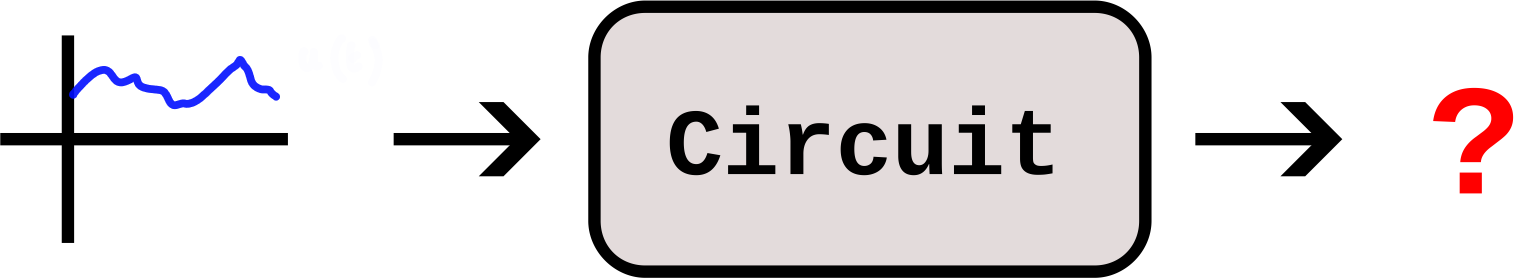
\includegraphics{part01/chap06/intro01.png}
\end{center}
	\caption{ Cas des signaux non analytiques}
\end{figure}

C'est ici qu'intervient la transformée de Fourier. Au lieu de travailler directement sur le signal d'entrée, la transformation de Fourier nous dit que tout signal peut être décomposé comme une somme de signaux "élémentaires" sinusoïdaux. Notre approche peut donc être simplifiée : au lieu de calculer directement la réponse d'un circuit à un signal temporel, nous allons décomposer ce signal en une somme de sinusoïdes, puis étudier comment le filtre altère chacune d'entre elles. \\

\begin{figure}[!h]
\begin{center}
\includesvg{part01/chap06/intro02}
\end{center}
	\caption{Principe de l'analyse harmonique}
\end{figure}

Nous pourrons alors reconstruire la réponse en sommant les réponses élémentaires. 

\section{Les séries de Fourier}

\subsection*{Définition}
\addcontentsline{toc}{subsection}{Définition}

Les séries de Fourier s'appliquent aux \textbf{\underline{fonctions périodiques}}. \\

Un signal périodique $s(t)$ de période $T$ peut, sous certaines conditions que nous supposerons toujours vérifiées en physique, se décomposer sous la forme suivante~:

\begin{equation}
	\bm{s(t) = a_0 + \sum_{n=1}^{\infty} \left(a_ncos\left( n\omega t\right) + b_nsin\left(n\omega t\right) \right)}
\end{equation}

Avec~: 

$$\omega=\dfrac{2\pi}{T}$$

et $a_0$, $a_n$, et $b_n$ des constantes~:

$$ a_0 = \dfrac{1}{T} \int_{0}^{T} s(t)dt $$

$$ a_n = \dfrac{2}{T} \int_{0}^{T} s(t)\,cos\left( n\omega t \right) dt \quad  \text{et} \quad b_n = \dfrac{2}{T} \int_{0}^{T} s(t)\,sin\left( n\omega t \right) dt $$  \\

\begin{itemize}
\item On peut remarquer que \textbf{le terme $a_0$ correspond à la valeur moyenne du signal}. \\

\item Les termes correspondant à $n=1$ sont appelés \textbf{le fondamental du signal}~:

$$ a_1\,cos\left( \omega t \right) + b_1\,sin\left( \omega t\right) $$  

\item Le terme général de rang $n$ est appelé \textbf{"harmonique de rang $n$"}~:

$$ a_n\,cos\left( n\omega t \right) + b_n\,sin\left( n\omega t\right) $$

\end{itemize}

\subsection*{Parité}
\addcontentsline{toc}{subsection}{Parité}

\begin{itemize}
\item Si la fonction s(t) est paire, tous les coefficients $b_n$ s'annulent :

$$ s(t) = \sum_{n=1}^{\infty} \left(a_ncos\left( n\omega t\right) \right) $$

\item Si la fonction s(t) est impaire, tous les coefficients $a_n$ s'annulent :

$$ s(t) = \sum_{n=1}^{\infty} \left(b_nsin\left(n \omega t\right) \right) $$

\end{itemize}

\subsection*{Forme phase-amplitude~:}
\addcontentsline{toc}{subsection}{Forme phase-amplitude}

Le terme général $a_n cos( n \omega t ) + b_n sin( n \omega t )$ peut être réécrit sous la forme : 

$$ a_ncos(n\omega t)+b_nsin(n\omega t) = \sqrt{a_n^2+b_n^2}\left(\dfrac{a_n}{\sqrt{a_n^2+b_n^2}}\,cos(n\omega t) + \dfrac{b_n}{\sqrt{a_n^2+b_n^2}}\,sin(n\omega t)\right)$$

Si on pose~:

$$c_n = \sqrt{a_n^2+b_n^2} \quad\text{,}\quad tan(\phi_n) = \dfrac{b_n}{a_n} \quad\text{et}\quad cos(\phi_n)= \dfrac{a_n}{\sqrt{a_n^2+b_n^2}}$$

On obtient~:

$$ a_ncos(n\omega t)+b_nsin(n\omega t) = c_n cos( n \omega t - \phi_n ) $$ 

Et le signal s'écrit alors~:

\begin{equation}
\bm{s(t)= a_0 + \sum_{n=1}^{\infty} c_n cos( n \omega t - \phi_n )} 
\end{equation}

Cette écriture, par rapport à la précédente, présente l'intérêt de représenter notre signal comme une somme de termes de forme unique, en cosinus avec phase et amplitude, plutôt que comme une somme de termes de deux formes différentes. \\

\textbf{\underline{Note}}~: Le lecteur attentif aura remarqué une correspondance entre les coordonnées $(a_n,b_n)$, qui correspondent aux coodonnées cartésiennes d'un vecteur 2D, et les coordonnées $(c_n, \phi_n)$ qui correspondent aux coordonnées polaires de ce même vecteur. Nous allons continuer, dans les chapitres à venir, à exploiter cette correspondance entre signal sinusoïdal et vecteur (ou nombre complexe).

\subsection*{Forme exponentielle}
\addcontentsline{toc}{subsection}{Forme exponentielle}

Une troisième forme existe pour les séries de Fourier. Il s'agit de la forme exponentielle qui s'écrit de la façon suivante~:

\begin{equation}
\bm{s(t) = \sum_{n=-\infty}^{\infty} d_n\,e^{jnwt} }
\end{equation}

Avec $j$ le nombre tel que $j^2=1$.

Dans cette forme, les coefficient $d_n$ sont des nombres complexes :

$$ d_n = \dfrac{1}{T} \int_{0}^{T} s(t)\,e^{ j\,n\,\omega\,t }\,dt \quad  \text{et donc} \quad d_n = 
\begin{cases} 
	\dfrac{a_n - j\,b_n}{2} & \text{si } n>0 \\
	\dfrac{a_n + j\,b_n}{2} & \text{si } n<0 \\
	a_0 & \text{si } n=0
\end{cases}
$$  

\subsection*{Spectre en fréquence }
\addcontentsline{toc}{subsection}{Spectre en fréquence}

Le spectre en fréquence d'un signal $s(t)$ est obtenu en représentant les coefficients $a_n$, $b_n$ ou $c_n$ par rapport aux pulsations correspondantes~: \\

\begin{center}
\includesvg[scale=0.5]{part01/chap06/spectre_en_frequence}
\end{center}

Cette représentation graphique permet de représenter la décomposition d'un signal en ses harmoniques et d'en comprendre les composantes. \\

\textit{Exemple: Le signal carré}\\

On considère le signal carré de période $T$ et d'amplitude $E$ suivant~: 

\begin{center}
\includesvg{part01/chap06/signal_carre}
\end{center}

Le signal est symétrique et centré verticalement. On a donc~:

$$a_0 = 0$$

De plus, on remarque que le signal est impair. Les coefficient $a_n$ sont donc nuls. \\ Il reste donc uniquement les termes $b_n$ :

$$ b_n = \dfrac{2}{T} \int_{-T/2}^{T/2} u(t)\,sin(n\omega t)dt = \dfrac{2E}{n\pi} \left( 1 - cos(n\pi) \right) $$

La décomposition ne comprend donc que des harmoniques d'ordre impaire car le terme en cosinus s'annule pour n pair.\\

\begin{minipage}{0.4\textwidth}
\begin{center}
\includesvg{part01/chap06/spectre_carre}
\end{center}
\end{minipage}
\begin{minipage}{0.5\textwidth}
	$$ u(t) = \dfrac{4E}{\pi}\left[ sin(\omega t) + \dfrac{1}{3} sin ( 3\omega t ) + \dfrac{1}{5} sin( 5 \omega t ) \dots \right] $$
\end{minipage}\\

\bigskip

Le spectre du signal carré est caractérisé par une décroissance de l'amplitude des harmoniques en $1/n$, ce qui constitue une décroissante très lente. Cela est typique des fonctions présentant une ou plusieurs discontinuités. 

\begin{figure}[!h]
\centering
\begin{subfigure}{0.4\textwidth}
\begin{center}
\begin{gnuplot}[terminal=epslatex, terminaloptions={color dashed size 8cm,5cm}]
set sample 1000
set xzeroaxis linetype -1
set xtics border nomirror
set ytics border nomirror
set border 3
set xr [-0.09:1]
set yr [-1.5:1.50]
T = 1 
f = 1/T
pi = 3.14159
w = 2*pi*f 
E = 1
u(n,x) = 2*E/(n*pi)*( 1 - cos(n*pi) ) * sin( n*w*x)
f(k,x)= sum [n=1:k] u(n,x)
plot \
	f(3,x) w l lc 4 lw 6 t ''
\end{gnuplot}
\end{center}
\caption{$N=3$}
\end{subfigure}
\hfill
\begin{subfigure}{0.4\textwidth}
\begin{center}
\begin{gnuplot}[terminal=epslatex, terminaloptions={color dashed size 8cm,5cm}]
set sample 1000
set xzeroaxis linetype -1
set xtics border nomirror
set ytics border nomirror
set border 3
set xr [-0.09:1]
set yr [-1.5:1.50]
T = 1 
f = 1/T
pi = 3.14159
w = 2*pi*f 
E = 1
u(n,x) = 2*E/(n*pi)*( 1 - cos(n*pi) ) * sin( n*w*x)
f(k,x)= sum [n=1:k] u(n,x)
plot \
	f(10,x) w l lc 4 lw 6 t ''
\end{gnuplot}
\end{center}
\caption{$N=10$}
\end{subfigure}
\hfill
\begin{subfigure}{0.4\textwidth}
\begin{center}
\begin{gnuplot}[terminal=epslatex, terminaloptions={color dashed size 8cm,5cm}]
set sample 1000
set xzeroaxis linetype -1
set xtics border nomirror
set ytics border nomirror
set border 3
set xr [-0.09:1]
set yr [-1.5:1.50]
T = 1 
f = 1/T
pi = 3.14159
w = 2*pi*f 
E = 1
u(n,x) = 2*E/(n*pi)*( 1 - cos(n*pi) ) * sin( n*w*x)
f(k,x)= sum [n=1:k] u(n,x)
plot \
	f(50,x) w l lc 4 lw 6 t ''
\end{gnuplot}
\end{center}
	\caption{$N=50$}
\end{subfigure}
\hfill
\begin{subfigure}{0.4\textwidth}
\begin{center}
\begin{gnuplot}[terminal=epslatex, terminaloptions={color dashed size 8cm,5cm}]
set sample 1000
set xzeroaxis linetype -1
set xtics border nomirror
set ytics border nomirror
set border 3
set xr [-0.09:1]
set yr [-1.5:1.50]
T = 1 
f = 1/T
pi = 3.14159
w = 2*pi*f 
E = 1
u(n,x) = 2*E/(n*pi)*( 1 - cos(n*pi) ) * sin( n*w*x)
f(k,x)= sum [n=1:k] u(n,x)
plot \
	f(100,x) w l lc 4 lw 6 t ''
\end{gnuplot}
\end{center}
	\caption{$N=100$}
\end{subfigure}
\end{figure}

\subsection*{Phénomène de Gibbs}
\addcontentsline{toc}{subsection}{Phénomène de Gibbs}
\begin{minipage}{0.4\textwidth}
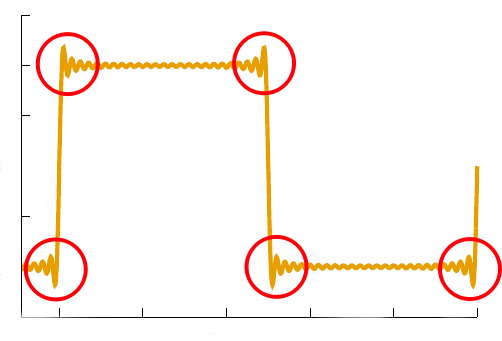
\includegraphics[width=\textwidth]{part01/chap06/gibbs.png}
\end{minipage}
\hfill
\begin{minipage}{0.5\textwidth}
\textbf{Le phénomène de Gibbs} est un effet de bord de la décomposition en séries de Fourier aux discontinuités. Ces "pics" oscillatoires (ringing) apparaissent en raison de l'approximation faite lorsque seules les N premières harmoniques du signal sont utilisées pour approximer un signal.\\

Lorsqu'un grand nombre d'harmoniques est pris en compte, cette erreur d'approximation converge vers une limite d'environ 9\% du changement de valeur.
\end{minipage}

\section{La transformée de Fourier}

La transformation de Fourier est une généralisation aux \textbf{\underline{fonctions non périodiques}} des séries de Fourier.

\subsection*{Définition}
\addcontentsline{toc}{subsection}{Définition}

La transformation de Fourier est une opération qui associe à chaque fonction intégrable sur ${\rm I\!R}$ une autre fonction décrivant le spectre fréquentiel de celle-ci. \\

Si elle existe, la transformée de Fourier de la fonction $f(t)$ s'écrit~:

\begin{equation*}
	\begin{split}
		\mathcal{F}(f): \, & \mathbb{R} \rightarrow  \mathbb{C}  \\	
		& \xi \mapsto F(\xi)=\int_{-\infty}^{+\infty}f(t)\,e^{-j\,\xi\,t}\,dt \\
	\end{split}
\end{equation*}

Cependant, cette écriture n'est pas unique et peut dépendre des conventions. Les physiciens notent souvent $\omega$ ou $2\pi\nu$ à la place de la variable complexe $\xi$ pour en faire les variables de pulsation ou de fréquence. L'équation précédente s'écrit alors ~: \\


\begin{equation}
	\begin{split}
		\mathcal{F}(f): \, & \mathbb{R} \rightarrow  \mathbb{C}  \\	
		& \nu \mapsto F(\nu)=\int_{-\infty}^{+\infty}f(t)\,e^{-j\,2\pi\nu\,t}\,dt \\
	\end{split}
\end{equation}

avec $\nu$ une fréquence en Hertz. \\

$F(\nu)$ indique la "quantité" de fréquence $\nu$ présente dans le signal $f(t)$ sur l'intervalle de temps $]-\infty;+\infty[$. \\

Il y a une équivalence entre donner $f(t)$ et donner $F(\nu)$ : ce sont deux descriptions équivalentes du même signal~:\\

\begin{itemize}

	\item L'une est \textbf{temporelle} : $f(t)$ \\

	\item L'autre est \textbf{fréquentielle} $F(\nu)$ \\

\end{itemize}

Cette notion est importante en electronique, car elle correspond à deux manières différentes d'analyser un circuit. Nous pouvons en effet nous intéresser aux phénomènes transitoires, et dans ce cas là l'approche temporelle est préférable. C'est par exemple ce que nous avons fait pour étudier la charge et la décharge d'un condensateur.

Mais nous pouvons aussi nous intéresser à ce qui se passse dans les différentes gammes de fréquence. Pour un ampli audio, par exemple, on cherche à savoir si les basses, par exemple, sont avantagées par rapport aux aigus. Dans ce cas là, une approche fréquentielle sera bien plus simple.

\subsection*{Spectre continu}
\addcontentsline{toc}{subsection}{Spectre continu}

Le lecteur averti aura -je n'en doute pas- remarqué que la fonction $F(\nu)$ est à valeur complexe. Elle admet : \\

\begin{itemize}
	\item \textbf{un spectre d'amplitude}~:  

		$$A_\xi = \lvert F(\nu) \rvert $$ 

	\item \textbf{un spectre de phase}~: 

		$$\phi(\xi) = arg(\,F(\nu)\,)$$ \\

\end{itemize}

Ces spectres sont \underline{continus}, à la différence des spectres obtenus par les séries de Fourier qui étaient composés de raies calculées aux multiples de la fréquence fondamentale.

\subsection*{Transformée de Fourier inverse }
\addcontentsline{toc}{subsection}{Transformée de Fourier inverse}

Si la fonction $F(\xi)$ est elle-même intégrable, il est possible de définir la réciproque de la transformation de Fourier, que l'on nomme "Transformation de Fourier inverse" et que l'on note $\mathcal{F}^{-1}$~:

\begin{equation*}
	f(t) = \mathcal{F}^{-1}(F)=\int_{-\infty}^{+\infty}F(\nu)\,e^{\,j2\pi\nu t}\,d\nu \\
\end{equation*}

Cette transformation inverse permet de repasser de la description fréquentielle à la description temporelle du signal. 

\vfill
\pagebreak
\subsection*{Propriétés de la transformée de Fourier}
\addcontentsline{toc}{subsection}{Propriétés de la transformée de Fourier}
\bigskip
\begin{itemize}
\item \textbf{Linéarité} 

\begin{equation}
a\,f_1(t)\,+\,b\,f_2(t) \leftrightarrow a\,F_1(\nu) + b\,F_2(\nu) 
\end{equation}

\item \textbf{Décalage temporel} 

\begin{equation}
f(t+t_0) \leftrightarrow e^{j2\pi\nu t_0}F(\nu)
\end{equation}

\item \textbf{Décalage fréquentiel} 

\begin{equation}
	e^{j2\pi\nu_0t}f(t) \leftrightarrow F(\nu-\nu_0)
\end{equation}

\item \textbf{Changement d'échelle} 

\begin{equation}
f(a\,t) \leftrightarrow \dfrac{1}{\left| a \right|} F\left( \dfrac{\nu}{a}\right)
\end{equation}

\item \textbf{Dérivation\footnote{Attention, la TF et la TF Inverse ne sont pas toujours définies !}}

\begin{equation}
	\dfrac{d\,f}{d\,t} \leftrightarrow j2\pi\nu\,F(\nu)
\end{equation}

\item \textbf{Primitive\footnote{Idem.}}

\begin{equation}
\int f(t)\,dt \leftrightarrow \dfrac{1}{j2\pi\nu}F(\nu)
\end{equation}

\item \textbf{Produit}

\begin{equation}
	f(t) \, g(t) \leftrightarrow \left( F \ast G \right)(\nu)
\end{equation}

\item \textbf{Produit de convolution}

\begin{equation}
\left( f \ast g\right)(t) \leftrightarrow F(\nu) \, G(\nu)
\end{equation}

\item \textbf{Inversion temporelle}

\begin{equation}
	f(-t) \leftrightarrow F(-\nu)
\end{equation}
	
\item \textbf{Conjuguaison complexe}
	\begin{equation}
		\overline{f}(t) \leftrightarrow \overline{F}(-\nu)
	\end{equation}

\pagebreak 
\item \textbf{Symétries}\\
\begin{itemize}
\item \textbf{ Dans le cas de signaux réels } \\

Si $f(t)$ est un signal réel~: $F(\nu) = F(-\nu)$ \\

Le spectre d'amplitude est alors une fonction paire, et le spectre d'argument une fonction impaire. \\

	\item \textbf{ Dans le cas de signaux imaginaires purs } \\
	
Si $f(t)$ est un signal imaginaire pur~: $F(\nu) = - F(-\nu)$ \\

\end{itemize}

\item{ \textbf{Parité}} \\

Si $f(t)$ est un signal réel et pair, alors $F(\nu)$ est réelle et paire. 

Si $f(t)$ est un signal réel et impair, alors $F(\nu)$ est imaginaire pure et impaire. 

\end{itemize}

\subsection*{Fourier et l'énergie des signaux}
\addcontentsline{toc}{subsection}{Fourier et l'énergie des signaux}

Lorsque les intégrales existent, on a~:

\begin{equation}
	\int^{+\infty}_{-\infty}\left|f(t)\right|^2\,dt = \int^{+\infty}_{-\infty} \left| F(\nu) \right| ^2 \, d\nu
\end{equation} 

\textbf{La transformée de Fourier conserve l'énergie du signal.} En conséquence, on peut définir une notion d'énergie par unité de fréquence, la \textbf{densité spectrale d'énergie (DSE)} du signal~:

\begin{equation}
	S_{xx}(\nu) = \left| F(\nu) \right|^2
\end{equation}

On peut alors définir \textbf{l'énergie dans une bande de fréquence} par l'intégrale de cette quantité sur une bande de fréquences~: \\
\begin{center}
\begin{minipage}{0.4\textwidth}
\begin{center}
\includesvg{part01/chap06/E_bandefreq}
\end{center}
\end{minipage}
\begin{minipage}{0.5\textwidth}
\begin{equation}
E_{\Delta\nu} = \int^{\nu_0+\Delta\nu/2}_{\nu_0-\Delta\nu/2} S_{xx}(\nu)\,d\nu
\end{equation}
\end{minipage}
\end{center}

Et donc l'\textbf{énergie totale du signal} peut s'écrire~:

\begin{equation}
E = \int^{+\infty}_{-\infty} S_{xx}(\nu)\,d\nu
\end{equation}

\pagebreak

\subsection*{Transformées de Fourier usuelles}
\addcontentsline{toc}{subsection}{Transformée de Fourier usuelles}
\bigskip
\begingroup
\setlength{\tabcolsep}{6pt} % Default value: 6pt
\renewcommand{\arraystretch}{2} % Default value: 1
\begin{center}
\begin{tabular}{|c|c|c|}
\hline
\textbf{Fonction} & \textbf{Représentation temporelle} & \textbf{Représentation fréquentielle} \\ 
\hline
\multirow{2}{*}{Constante} & $1$ & $\delta(\nu)$ \\
& \includesvg{part01/chap06/tf_constante_t} 
& \includesvg{part01/chap06/tfgraph}\\
\hline
\multirow{2}{*}{Sinus} & $sin(2\pi\nu_0t+\phi_0)$ & $\dfrac{1}{2j}\,(e^{j\phi_0}\,\delta(\nu-\nu_0) - e^{-j\phi_0}\,\delta(\nu+\nu_0))$ \\
& \includesvg{part01/chap06/tf_sinus_t} 
& \includesvg{part01/chap06/tfgraph}\\
\hline
\multirow{2}{*}{Cosinus} & $cos(2\pi\nu_0t+\phi_0)$ & $\dfrac{1}{2}\,(e^{j\phi_0}\,\delta(\nu-\nu_0) + e^{-j\phi_0}\,\delta(\nu+\nu_0))$ \\
& \includesvg{part01/chap06/tf_cosinus_t} 
& \includesvg{part01/chap06/tfgraph}\\
\hline
\multirow{2}{*}{Sinus cardinal} & $sinc(t) = \dfrac{sin(t)}{t}$ & $ \Pi_{2\nu_0}(\nu) $ \\[2ex]
& \includesvg{part01/chap06/tf_sinus_card_t} 
& \includesvg{part01/chap06/tfgraph}\\
\hline
\multirow{2}{*}{Dirac} & $\delta(t)$ & $1$ \\
& \includesvg{part01/chap06/tfgraph} 
& \includesvg{part01/chap06/tf_dirac_f}\\
\hline
\end{tabular}
\end{center}

\pagebreak

\begin{center}
\begin{tabular}{|c|c|c|}
\hline
\textbf{Fonction} & \textbf{Représentation temporelle} & \textbf{Représentation fréquentielle} \\ 
\hline
\multirow{2}{*}{Dirac décalé en $t_0$ } & $\delta(t)=\delta(t-t_0)$ & $e^{-j\,2\pi\nu t_0}$ \\
& \includesvg{part01/chap06/tfgraph} 
& \includesvg{part01/chap06/tfgraph}\\
\hline
\multirow{2}{*}{Exponentielle complexe} & $e^{j2\pi \nu_0 t}$ & $\delta(\nu-\nu_0)$ \\
& \includesvg{part01/chap06/tfgraph} 
& \includesvg{part01/chap06/tfgraph}\\
\hline
\multirow{2}{*}{Peigne de Dirac} & $\Sha_{T_e}(t)$ & $\Sha_{F_e}(\nu)$ \\
& \includesvg{part01/chap06/tfgraph} 
& \includesvg{part01/chap06/tfgraph}\\
\hline
\multirow{2}{*}{Fonction porte} & $\Pi_{T_0/2}$ & $ T_0\,sinc(\pi\nu T_0)$ \\
& \includesvg{part01/chap06/tfgraph} 
& \includesvg{part01/chap06/tfgraph}\\
\hline
\end{tabular}
\end{center}

\endgroup


%\part{ Analyse harmonique }
%\part{ Les semi-conducteurs }
%\input{ diode.tex }
%\input{ bjt.tex }
%\input{ fet.tex }


\part{Annexes}
\appendix

\chapter{Les unités}

\section{Les unités S.I.}

Les septs unités du système SI sont les unités à partir desquelles on peut contruire toutes autres unités en physiques. Ces sept unités de bases sont les suivantes~:

\begin{center}
\bgroup
\def\arraystretch{1.2}%  1 is the default, change whatever you need
\rowcolors{2}{blue!30}{blue!10}
\begin{tabular}{|c c c|}
	\hline
	\textbf{Symbole} & \textbf{Nom} & \textbf{Usage} \\
	\hline
	\hline
	m & Mètre & Longueur \\
	kg & Kilogramme & Masse \\
	s & Seconde & Temps \\
	A & Ampère & Intensité de Courant électrique \\
	K & Kelvin & Température \\
	cd & Candela & Intensité lumineuse \\
	mol & Mole & Quantité de matière \\
	\hline
\end{tabular}
\egroup
\end{center}

\section{Les unités courantes en electronique}
\begin{center}
\bgroup
\def\arraystretch{1.2}%  1 is the default, change whatever you need
\rowcolors{2}{blue!30}{blue!10}
\begin{tabular}{|c c c c|}
	\hline
	\textbf{Symbole} & \textbf{Nom} & \textbf{Usage} & \textbf{Unités SI}  \\
	\hline
	\hline
	C & Coulomb & Charge & $A\,s$ \\
	F & Farad & Capacité électrique & $m^{-2}\,kg^{-1}\,s^{4}\,A^{2}$ \\
	H & Henry & Inductance & $m^2\,kg\,s^{-2}\,A^{-2}$ \\
	Hz & Hertz & Fréquence & $s^{-1}$ \\
	S & Siemens & Conductance, Admittance, Suceptance & $m^{-2}\,kg^{-1}\,s^{3}\,A^{2}$ \\
	J & Joule & Energie, Travail, Quantité de chaleur & $kg\,m^2\,s^{-2}$  \\
	V & Volt & Force electromotrice, Potentiel & $kg\,m^{2}\,s^{-3}\,A^{-1}$  \\
	W & Watt & Puissance, Flux energétique & $kg\,m^2\,s^{-3}$$kg\,m^2\,s^{-3}$ \\
	$\Omega$ & Ohm & Résistance & $m^2\,kg\,s^{-3}\,A^2$ \\
	\hline
\end{tabular}
\egroup
\end{center}

\section{Les multiples}
\smallskip
\begin{center}
\bgroup
\def\arraystretch{1.2}%  1 is the default, change whatever you need
\rowcolors{2}{blue!30}{blue!10}
\begin{tabular}{|p{0.1\textwidth}>{\centering}p{0.1\textwidth}>{\centering\arraybackslash}p{0.1\textwidth}|}
	\hline
	\textbf{Facteur} & \textbf{Nom} & \textbf{Symbole}  \\
	\hline
	\hline
	$10^{-30}$ & quecto & q \\
	$10^{-27}$ & ronto & r \\
	$10^{-24}$ & yocto & y \\
	$10^{-21}$ & zepto & z \\
	$10^{-18}$ & atto & a \\
	$10^{-15}$ & femto & f \\
	$10^{-12}$ & pico & p \\
	$10^{-9}$ & nano & n \\
	$10^{-6}$ & micro & $\mu$ \\
	$10^{-3}$ & milli & m \\
	$10^{-2}$ & centi & c \\
	$10^{-1}$ & deci & d \\
	\textbf{1} & \textbf{unité} & \\
	$10^{1}$ & deca & da \\
	$10^{2}$ & hecto & h \\
	$10^{3}$ & kilo & k \\
	$10^{6}$ & mega & M \\
	$10^{9}$ & giga & G \\
	$10^{12}$ & tera & T \\
	$10^{15}$ & peta & P \\
	$10^{18}$ & exa & E \\
	$10^{21}$ & zetta & Z \\
	$10^{24}$ & yotta & Y \\
	$10^{27}$ & ronna & R \\
	$10^{30}$ & quetta & Q \\
	\hline
\end{tabular}
\egroup
\end{center}


\chapter{Résolution d'une EDO d'ordre 1}

%TODO

\chapter{Résolution d'une EDO d'ordre 2}
\label{annexe:edo2}

%TODO

\chapter{Résolution d'une EDO d'ordre 1}

%TODO

\chapter{Résolution d'une EDO d'ordre 2}
\label{annexe:edo2}

%TODO


\backmatter

\phantomsection
\cleardoublepage
\addcontentsline{toc}{part}{\indexname}
\printindex

% Fin du document
\end{document}

